\documentclass{report}
\usepackage{natbib}
\usepackage{tikz}
\title{Adequacy of PCF}
\usepackage{mathpartir}
\usepackage{amsmath}
\usepackage{parskip}
%\usepackage{bbold}
\usepackage{color}
\usepackage{amssymb}
\usepackage{stmaryrd}
\newcommand{\rel}{\sqsubseteq_{C}}
\usepackage{amsthm}
\newtheorem{thm}{Theorem}
\newtheorem{lem}{Lemma}
\newtheorem{cor}{Corollary}
\usepackage{changepage}
\author{Natalie Ravenhill}
\begin{document}
\maketitle
\newcommand{\natb}{\mathbb{N}_{\bot}}
\tableofcontents
\chapter{Introduction}
%Literature Review goes here

\chapter{Background}
There are some mathematical topics and proof techniques, which are very important in semantics, that we need for this project. To prove Adequacy, we need a model for our language in which we can work in.

We can use sets to model each type in PCF. But for function types,if a function of that type never terminates, then its result will not be in the set. Therefore we need an additional element in the model to represent this.

We also want to compare different programs in the model, which we can do by an information ordering, where more defined programs are higher in the ordering and the element representing non-termination is the lowest. This ordering is a partial order.

%define and give example.

Therefore, we need a structure which includes a set, an ordering on the set and an undefined element - this is a domain.

The usefulness of this ordering will become apparent when we discuss recursion (see \ref{fixpoint}).

%Recursion also gives an issue of what functions we can define in the model. As described in \citep{streicher06}, if a function of type  $A \to B$ are represented in the model by all the functions between the domains of the types, then every function would have to have a fixpoint. In reality, only monotone functions have fixpoints. Therefore we must restrict the functions to those with fixpoints. 

\section{Domain Theory}\label{dom}
There is an entire area of mathematics devoted to exploring these structures called Domain Theory, as described in \citep{Gunter92} and  \citep{Hutton14}.

Generally domains can be defined in two different ways, either by using chains or by using directed sets.

\vspace{0.5cm}

\begin{defn}
A \textbf{chain} is a sequence $x_0 \sqsubseteq x_1 \sqsubseteq x_2 \sqsubseteq \dots $ where every element is larger than the preceding one.

\vspace{0.5cm}

Formally we define a chain as a function $\mathbb{N} \to X$, such that if $i \leq j$ then $x_i \sqsubseteq x_j$
\end{defn}

As an example, given the lifted set  $\natb$ (a set with $\bot$ added) then a chain can be formed in three ways:

\begin{itemize}
\item{$\bot \sqsubseteq \dots \sqsubseteq \bot$, for any number of $\bot$s}
\item{$n \sqsubseteq \dots \sqsubseteq n$, for any number of $n$s, where $n$ is the same number each time}
\item{$\bot \sqsubseteq \dots \sqsubseteq \bot \sqsubseteq n \sqsubseteq \dots \sqsubseteq n$, for any number of $\bot$s followed by any number of identical $n$s}
\end{itemize}

This is because the ordering on the lifted set is only defined between numbers and themselves, so it only contains $\bot \sqsubseteq \bot$ and $\bot \sqsubseteq n$ for some $n \in \mathbbm{N}$.

\vspace{0.5cm}
 
\begin{defn}
A \textbf{directed set} $X$, is a non-empty set where

\[ \forall x,y \in X. \ \exists z \in X. \ x \sqsubseteq z \ \wedge y \ \sqsubseteq z \]
\end{defn}

Domains can be defined using either of these structures.  If we take all the elements in a chain as a set, then the least upper bound will be the value of $z$ for any two elements of the set. Therefore a chain is an example of a directed set.


For the rest of the report, we use the definition of domains that uses chains, as opposed to directed sets.
\vspace{0.5cm}
%\section{Definition of a domain}
\begin{defn}
A domain ($X, \bot, \sqsubseteq$) consists of a set $X$, an element $\bot$ and a relation $\sqsubseteq \ \subseteq X_\bot \times X_\bot$ such that:

\begin{itemize}
\item{$\forall x \in X. \ \bot \sqsubseteq X$}
\item{$\sqsubseteq$ is a partial order}
\item{All chains of elements of $X_\bot$ have a limit (i.e.\ a least upper bound). To prove this there are two properties we must prove, for some $z \in X_\bot$}
\begin{itemize}
 \item{$\forall i. x_i \sqsubseteq z$ \hspace{1cm} \emph{($z$ is the upper bound)}}
 \item{$\forall y. (\forall i.x_i  \sqsubseteq y) \Rightarrow \ z \sqsubseteq y$ \hspace{0.25cm} \emph{($z$ is the least upper bound)}}
\end{itemize}
\end{itemize}

The limit of a chain is usually written as $\bigsqcup x_n$, where $x_n$ is a chain of length $n$ and $x_i$ is the element at the $i$th position in the chain.

\end{defn} 

\section{Examples of Domains}\label{ex}
\subsection{Single Element Domain}\label{single}
In a single element domain the underlying set is $\{x\}$, so the only element $\bot$ can be is $x$ and $\sqsubseteq$ just contains the pair $(x,x)$

\vspace{0.5cm}

\begin{lem}
$(\{x\},x,\sqsubseteq)$ is a domain.
\end{lem}

\begin{proof}
We prove the three conditions in the domain definition to show that $(\{x\},x,\sqsubseteq)$ is a domain).

There is only one element, $x$, and $x \sqsubseteq x$ is in the ordering, so $\forall x \in \{x\}. \ x \sqsubseteq x$.

Next, we prove $\sqsubseteq$ is a partial order. As the only element in the underlying set is $x$ and $x \sqsubseteq x$ is in the ordering, then it must be  reflexive. We can only have $x \sqsubseteq x$ in the ordering and $x = x$, so it is antisymmetric.
Any $x,y$ and $z$ must all be $x$ and $x \sqsubseteq x$ is in the ordering, so $\sqsubseteq$ is transitive. Therefore $\sqsubseteq$ is a partial order.


Finally, we prove that all chains must have a least upper bound. As $x$ is the only possible element, all chains will be of the form 

\[ x \sqsubseteq x  \sqsubseteq x  \sqsubseteq \dots \]

Let $z = \bigsqcup x_n = x$. Then the only possible $x_i$ is $x$, so we must have $x \sqsubseteq x$. This is in the ordering. Therefore $\forall i. x_i \sqsubseteq x$.

Then we prove $\forall y. (\forall i . x_i \sqsubseteq y) \Rightarrow x \sqsubseteq y$. The only possible value of $y$ is $x$. Therefore we must have $x \sqsubseteq x$, which is in the ordering.

\vspace{0.25cm}

Now we have proved all the conditions, so the single element domain is a domain.
\end{proof}

\subsection{Flat Natural Numbers}\label{flat} A domain is a \textbf{flat} domain if  the only ordering is between $\bot$ and the elements of the underlying set. In this example the underlying set is  $\mathbbm{N}$, the set of natural numbers, so the only orderings we have are $\bot \sqsubseteq 0$, $\bot \sqsubseteq 1$, $\bot \sqsubseteq 2$, etc... 

Therefore the relation is defined as:

\[ \sqsubseteq  \ = \{ (\bot , \bot) \} \cup \{ (\bot , n) , (n ,n) \ | \ n \in \mathbbm{N} \} \] 

which gives us the following picture:   

\vspace{0.5cm}

\begin{center}
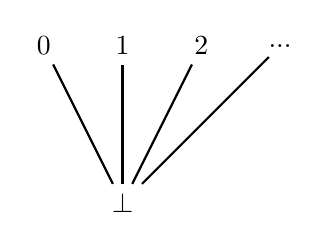
\begin{tikzpicture}
    \node (top) at (0,0) {$\bot$};
    \node (a) at (-1,2) {0};
    \node (b) at (0,2) {1};
    \node (c) at (1,2) {2};
    \node (d) at (2,2) {...};
    \draw [thick] (top) -- (a);
    \draw [thick] (top) -- (b);
    \draw [thick] (top) -- (c);
    \draw [thick] (top) -- (d);
\end{tikzpicture}
\end{center}

\vspace{0.5cm}

Now we must prove that this is a domain:

\vspace{0.5cm}

\begin{lem}
$(\mathbbm{N}, \bot, \sqsubseteq)$ is a domain.
\end{lem} 

\begin{proof}
We prove the three conditions in the domain definition:

In the definition of our relation we have $\{ (\bot , n) \ | \ n \in \mathbb{N} \}$, so $\forall x \in \mathbb{N}. \ \bot \sqsubseteq x$.

Next, we prove $\sqsubseteq$ is a partial order. From the  definition of $\sqsubseteq$, we have $\{(x,x) \ | \ x \in \natb \}$, which is a subset of $\sqsubseteq$, so $\sqsubseteq$ must be reflexive.

We prove antisymmetry by case analysis. When $x = \bot$, the only possible $y$ we can have such that $y \sqsubseteq x$ is $y = \bot$, as  $n \sqsubseteq \bot$ is not defined in the relation for any $n$. Therefore $x = y = \bot$. When $x = n$, the only possible value of $y$ is $n$, so $x = y = n$. Therefore every element of the underlying set satisfies antisymmetry.

We also prove transitivity by case analysis. If $x = \bot$ and $y =n$, then we must have $z = n$ for $(y,z)$ to be in $\sqsubseteq$. Then we need $\bot \sqsubseteq n$ , which we have, as $(\bot, n)$, for any $n \in \mathbb{N}$ is defined in the relation. If $x = \bot = y$, then we have two options for $z$. When $z = n$, we should have $\bot \sqsubseteq n$, which we have, as $(\bot, n)$ for any $n \in \mathbb{N}$ is defined in the relation. When $z = \bot$, we want $ \bot \sqsubseteq \bot$, which is also in the definition of $\sqsubseteq$. If $x = n$, then both $y$ and $z$ must also be equal to $n$ for $x \sqsubseteq y$ and $y \sqsubseteq z$ to be defined. Therefore we should  have $n \sqsubseteq n$. This is in the definition of $\sqsubseteq$.

Finally we prove that all chains must have a least upper bound. We prove this by case analysis on the different chains. For  chains of the form $\bot \sqsubseteq \dots \sqsubseteq \bot$, let $z = \bot$. The last element in the chain will always be $\bot$, so for every $i$ we have $\bot \sqsubseteq \bot$. Therefore $\forall i . x_i \sqsubseteq \bot$.
For the second statement, as every element is $\bot$, $x_i = \bot$ and $y = \bot$, we have $\bot \sqsubseteq \bot$ for $z \sqsubseteq y$. Therefore $\forall y. (\forall i . x_i \sqsubseteq y) \Rightarrow \bot \sqsubseteq y$ holds.

For chains of the form $n \sqsubseteq \dots \sqsubseteq n$, let $z = n$. The last element in the chain will always be $n$, so for every $n$ we have $n \sqsubseteq n$. Therefore $\forall i . x_i \sqsubseteq n$. For the second part, every element is $n$, so $x_i = n$ and $y = n$. Then we have $n \sqsubseteq n$ for $z \sqsubseteq y$. Therefore $\forall y. (\forall i . x_i \sqsubseteq y) \Rightarrow n \sqsubseteq y$ holds.

For chains of the form $\bot \sqsubseteq \dots \sqsubseteq \bot \sqsubseteq n \sqsubseteq \dots \sqsubseteq n$, let $z = n$.  The last element will be $n$. We have both $\bot \sqsubseteq n$ and $n \sqsubseteq n$ in the relation, so for any $x$, we have $x \sqsubseteq n$. Therefore $\forall i . x_i \sqsubseteq n$. For the second part, $(\forall i . x_i \sqsubseteq y)$ is only true when $y = n$, so we only have to consider this case. Then we have $n \sqsubseteq n$ for $z \sqsubseteq y$. Therefore $\forall y. (\forall i . x_i \sqsubseteq y) \Rightarrow n \sqsubseteq y$ holds.
\end{proof}

\subsection{Product of domains}\label{prod}
Given two domains $\mathbb{X} = (X, \bot_X, \sqsubseteq_X)$ and $\mathbb{Y} = (Y, \bot_Y, \leq_Y)$, we have a new domain,  where $X \times Y$ is the underlying set, the bottom element is $(\bot_X, \bot_Y)$ and $(x,y) \sqsubseteq (x',y')$ is defined when $x \sqsubseteq_X x'$ and $y \leq_Y y'$ are defined.

\vspace{0.25cm}

Now we must prove that this is a domain.

\vspace{0.5cm}

\begin{lem}
$(X \times Y, (\bot_X, \bot_Y), \sqsubseteq)$ is a domain
\end{lem}

\begin{proof}
We prove the three conditions in the domain definition:

As $\mathbbm{X}$ is a domain, we know $\forall x \in X. \ \bot_X \sqsubseteq_X x$ and because $\mathbb{Y}$ is a domain, we know $\forall y \in Y. \ \bot_Y \leq_Y y$. Therefore we have $\forall x,y . \ \bot_X \sqsubseteq_X x \wedge \bot_Y \leq_Y y$. This is the same as $\forall (x,y) \in X \times Y. (\bot_X,\bot_Y) \sqsubseteq (x,y)$.

Next, we prove $\sqsubseteq $ is a partial order. For an element $(x,y) \in X \times Y$, we have $x \sqsubseteq_X x$ and $y \leq_Y y$ because $\mathbb{X}$ and $\mathbb{Y}$ are domains, so their orderings are reflexive. This means we have $(x,y) \sqsubseteq (x,y)$, so $\sqsubseteq$ is also reflexive. For elements $(x,y)$ and $(x',y')$ we can assume $(x,y) \sqsubseteq (x',y')$ and $(x',y') \sqsubseteq (x,y)$. Expanding these definitions we have $x \sqsubseteq_X x' \wedge y \leq_Y y' \wedge x' \sqsubseteq_X x \wedge y' \leq_Y y$. If we reorder this we have:

\[x \sqsubseteq_X x' \wedge x' \sqsubseteq_X x \wedge y \leq_Y y' \wedge y' \leq_Y y \]

As the orderings on $\mathbb{X}$ and $\mathbb{Y}$ are antisymmetric, we can rewrite this as $x = x'$ and $y = y'$. Therefore we have $(x,y) = (x',y')$, so $\sqsubseteq$ is antisymmetric. For elements $(x,y), (x',y')$ and $(x'',y'')$ we can assume $(x,y) \sqsubseteq (x',y')$ and $(x',y') \sqsubseteq (x'',y'')$. Expanding these definitions gives us $x \sqsubseteq_X x' \ \wedge \ y \leq_Y y' \wedge \ x' \sqsubseteq_X x'' \wedge y' \leq_Y y''$. If we reorder this we have:


\[x \sqsubseteq_X x' \wedge x' \sqsubseteq_X x'' \wedge y \leq_Y y' \wedge y' \leq_Y y'' \]

As the orderings on $\mathbb{X}$ and $\mathbb{Y}$ are transitive, we can rewrite this as $x \sqsubseteq_X x''$ and $y \leq_Y y''$. Therefore we can now define $(x,y) \sqsubseteq (x'',y'')$, so $\sqsubseteq$ is transitive.

Finally we prove that all chains have a least upper bound. Chains of $\mathbbm{X \times Y}$ will be of the form:

\[(x,y) \sqsubseteq (x', y') \sqsubseteq (x'', y'') \sqsubseteq \dots \]

where $x \sqsubseteq_X x' \sqsubseteq_X x'' \dots$ and $y \leq_Y y' \leq_Y y'' \dots $.

Let $z = \bigsqcup (x, y)_n = (\bigsqcup x_n, \bigsqcup y_n)$. Then as $\mathbb{X}$ and $\mathbb{Y}$ are domains, we have $\forall i. \ x_i \sqsubseteq_X \bigsqcup x_n$ and  $\forall i. \  y_i \leq_Y \bigsqcup y_n$. Therefore, for any $(x,y)$ we have $\forall i. (x_i ,y_i) \sqsubseteq (\bigsqcup x_n , \bigsqcup y_n)$.

%\item{$\forall (x',y'). \ (\forall i . (x_i,y_i) \sqsubseteq (x',y')) \Rightarrow z \sqsubseteq (x',y')$\\
As $\mathbb{X}$ and $\mathbb{Y}$ are domains, we have $\forall x'. \  (\forall i.\  x_i \sqsubseteq_X x') \Rightarrow \bigsqcup x_n \sqsubseteq_X x'$ and $\forall y'. \ (\forall i. \ y_i \leq_Y y') \Rightarrow \bigsqcup y_n \leq_Y y'$.

 Therefore if we assume $\forall (x',y'). (\forall i . (x_i,y_i) \sqsubseteq (x',y'))$, then we know $\bigsqcup x_n \sqsubseteq_X x'$ and $\bigsqcup y_n \leq_Y y'$. This is the definition of $(\bigsqcup x_n , \bigsqcup y_n) \sqsubseteq (x',y')$.

\vspace{0.25cm}

Now we have proved all the conditions, so the product of two domains is also a domain.
\end{proof}

\section{Monotone and Continuous Functions}
There are two different types of functions that we will use when modelling PCF functions:

\vspace{0.25cm}

\begin{defn}
A \textbf{monotone} function, $f$, is a function that preserves the order of a partially ordered set, $X$,  so:

\[ \forall x, y \in X. \ x \sqsubseteq y  \Rightarrow f(x) \sqsubseteq f(y) \]
\end{defn}

Given a chain $x_0 \sqsubseteq x_1 \sqsubseteq \dots$, we can form the chain $f(x_0) \sqsubseteq f(x_1) \sqsubseteq \dots$ using a monotone function.

\vspace{0.25cm}

\begin{defn}
A \textbf{continuous} function $f$ is a function which when applied to the limit of a chain gives the same result as the limit of the chain formed by applying $f$ to every element of another chain. Formally:

\[ f(\bigsqcup x_n) = \bigsqcup (f(x_n))\]
\end{defn}

Therefore continuous functions must also be monotone:

\vspace{0.25cm}

\begin{thm}\label{mono}
Continuous functions are monotone
\end{thm}

\begin{proof}
Given a continuous function $f$, on a partially ordered set $X$, we need to show that $\forall x,y \in X. \ x \sqsubseteq y \Rightarrow f(x) \sqsubseteq f(y)$.
Assume we have a chain $x_n$, where $x_0 = x$ and $x_{n + 1} = y$ for all $n$:

\[x \sqsubseteq y \sqsubseteq y \dots \] .

The limit of this chain will be $y$, so $f(\bigsqcup x_n) = f(y) = \bigsqcup (f (x_n))$.

We also know that because there are only two different elements in the chain, $\bigsqcup (f (x_n)) = f(x) \sqcup f(y) = f(y)$, so therefore $f(x) \sqsubseteq f(y)$.

\end{proof}

\subsection{Domain of Continuous Functions}\label{cont}

We can form a domain of continuous functions between two other domains:

Given two domains $\mathbb{X} = (X, \bot_X, \sqsubseteq_X)$ and $\mathbb{Y} = (Y, \bot_Y, \leq_y)$, we can form the set $\cont(X,Y) =\{ f : X \to Y\}$, of continuous functions between the underlying sets, where:

\begin{itemize}
\item{$\forall x, x' \in X. \ x \sqsubseteq_X x' \Rightarrow f(x) \leq_Y f(x')$ \hspace{1cm} $f$ preserves the ordering of chains in $\mathbbm{X}$}
\item{$x_n \in \chain(X) \Rightarrow f(\bigsqcup x_n) = \bigsqcup f(x_n)$ \hspace{2cm} $f$ is continuous}
\end{itemize} 

where $\chain(X)$ is the set of all possible chains we can form from  $\mathbbm{X}$.

$\bot_{X \to Y}$ is defined as the function $\bot = \lambda x. \bot (x)$, the function that loops on all inputs. The output of this function will always be $\bot$, because it does not terminate. 

The relation $\rel$ is defined as

\[ \rel  \ = \{ (f , g) \ | \ f,g \in \cont(X,Y) \ \wedge \ \forall x \in X. \ f(x) \leq_Y g(x)\} \]

Therefore our domain will be $(\cont(X,Y), \bot_{X \to Y}, \sqsubseteq_C)$. Now we must prove that this is a domain.

\vspace{0.5cm}

\begin{lem}
$(\cont(X,Y), \bot_{X \to Y}, \sqsubseteq_C)$ is a domain.
\end{lem}

\begin{proof}
We must prove the three conditions in the domain definition:

For all $x \in X$ we have $\bot \leq_Y f(x)$. As $\mathbb{Y}$ is a domain we know this holds for every element of $Y$ and as the codomain of $f$ is $Y$, every $f(x)$ is in $Y$. Therefore $\forall f \in \cont(X,Y). \ \bot_{X \to Y} \rel f$.

Next we prove $\rel$ is a partial order. As $\mathbb{Y}$ is a domain, we know that $\leq_Y$ is a partial order. For reflexivity, we need to prove that $\forall f \in \cont(X,Y). \ f \rel f$. We can rewrite this using the definition of $\rel$ to get 
\[\forall f \in \cont(X,Y). \ (\forall x \in X. \ f(x) \leq_Y f(x))\]
 Functions are single valued, so we know $\forall f. \ \forall x. \ f(x) = f(x)$ and as $\leq_Y$ is reflexive we know $\forall f. \forall x \in X. \ f(x) \leq_Y f(x)$. Therefore we have $f \rel f$, for any $f \in \cont(X,Y)$. For antisymmetry, we need to prove that $\forall f,g \in \cont(X,Y). \ ((f \rel g) \ \wedge \ (g \rel f)) \Rightarrow f = g$. Rewriting this using the definition of $\rel$ gives us
 \[\forall f,g \in \cont(X,Y). \ (\forall x \in X. \ ((f(x) \leq_Y g(x)) \ \wedge \ (g(x) \leq_Y f(x))) \Rightarrow f(x) = g(x))\] 
 $\leq_Y$ is antisymmetric, so we have $\forall x \in X. \ f(x) = g(x)$, for any values of $f$ and $g$. Therefore $\rel$ is also antisymmetric. For transitivity, we need to prove that $\forall f,g,h \in \cont(X,Y). \ ((f \rel g) \  \wedge \ (g \rel h)) \Rightarrow f \rel h$. Rewriting this using the definition of $\rel$ gives us 

\[\forall f,g,h \in \cont(X,Y). \ (\forall x \in X. \ ((f(x) \leq_Y g(x)) \ \wedge \ (g(x) \leq_Y h(x))) \Rightarrow f(x) \rel h(x)) \]
 
As $\leq_Y$ is transitive, we have $\forall x \in X.f(x) \leq_Y h(x)$, for all $f, g$ and $h$. Therefore $\rel$ is also transitive. 

Finally we prove that all chains have a least upper bound. Let $z = \lambda x. \bigsqcup^Y f_n (x)$, where $\bigsqcup^Y f_n (x)$ is the limit of the chain (in $\mathbbm{Y}$) obtained by applying the functions in some chain of elements of $\cont(X,Y)$ to a certain element $x \in X$.

An example of a chain of such functions is:

\[ f_1 \rel f_2 \rel \dots \rel \bigsqcup f_n \]

If we expand this using the definition of $\rel$ we have

\[ \forall x \in X. \ (f_1(x) \leq_y f_2(x) \leq_Y \dots \leq_Y \bigsqcup f_n (x)) \]

This is a set of chains in $\chain(Y)$ where every chain contains the result of each function on a certain $x \in X_\bot$. As $\mathbb{Y}$ is a domain, the least upper bound is defined for any chain using the elements of $Y_\bot$. Therefore we know that the least upper bound $\bigsqcup f_n (x)$ is defined. Now we can see that this is the same as our definition of $z$, which was $\lambda x. \bigsqcup^Y f_n (x)$.

For the second part of the proof, we can rewrite it using the definition of $\rel$ as

\[ \forall x \in X. \ (\forall g. (\forall i . f_i(x) \leq_Y g(x)) \Rightarrow z(x) \leq_Y g(x)) \]


As $\mathbbm{Y}$ is  a domain, $(\forall i . f_i(x) \leq_Y g(x)) \Rightarrow z(x) \leq_Y g(x))$ holds for each of our individual chains for each $x \in X$. Therefore we have $ \forall g. (\forall i . f_i \rel g) \Rightarrow z \rel g$
\end{proof}


\section{Fixpoint Theorem}\label{fixpoint}

Now we have a domain of continuous functions, we can use it to state and prove the fixpoint theorem. The following theorem is an important result in recursion theory, that we will use to model recursion in PCF. The chain given in the theorem is the chain obtained by repeatedly iterating a recursive function on its previous result, starting with $\bot$. If an input of the function is computed using $f^n(\bot)$ and it needs more than $n$ iterations then it will not terminate. As the chain can be infinitely long, it can model infinite (general) recursion.

\vspace{0.5cm}


\begin{thm}
Every continuous function $f : X \to X$ has a least fixpoint, which is the limit of the chain $\bot \sqsubseteq f(\bot) \sqsubseteq f^2(\bot) \sqsubseteq \dots$
\end{thm}

\begin{proof}
 Define the fixpoint function $fix(f) \equiv \bigsqcup f^n (\bot)$. This is the limit of the chain in the theorem. We know this limit exists because $f$ is continuous, so $(X, \bot, \sqsubseteq)$ must form a domain (see Section \ref{cont}), and by the definition of domain, all chains of $\mathbbm{X}$ have a limit. 

%First we must prove that this limit exists, so $\forall i \in \mathbb{N} . \ f^i(\bot) \sqsubseteq f^n(\bot)$. We prove this by induction. If $i = 0$, then the only element of the chain is $f^0(\bot) = \bot$. $\bot$ is the least element of the chain, so we have $\bot  \sqsubseteq f^n(\bot)$. 

%The inductive hypothesis is $\sqcup f^i(\bot)$ exists. Applying $f$ to this gives us $f(\sqcup f^i(\bot))$. $f$ is continuous, so this is equal to $\sqcup f(f^i(\bot)) = \sqcup f^{i+1}(\bot) $

\paragraph{$\bigsqcup f^n (\bot)$ is a fixpoint}
For the limit to be a fixpoint we must have  $f( \bigsqcup f^n (\bot)) =  \bigsqcup f^n (\bot)$.  As $f$ is continuous, we have $f( \bigsqcup f^n (\bot)) = \bigsqcup f(f^n(\bot)) = \bigsqcup f^{n+1}(\bot)$. The chain formed by $f^{n+1}$ is $f(\bot)  \sqsubseteq f^2(\bot) \sqsubseteq \dots$. This is the same as our original chain, but without $\bot$ at the start. Because $\mathbbm{X}$ is a domain, we know that $\forall x \in X. \ \bot \sqsubseteq x$. Therefore $\bot$ has no effect on the limit because every element is higher than it, so removing $\bot$ will not change the limit. This means that $\bigsqcup f^{n+1} (\bot) = \bigsqcup f^n(\bot)$.

\paragraph{$\bigsqcup f^n (\bot)$ is the least fixpoint}
Let $x$ be an element of our chain such that $fix(x) = x$. Then for $\bigsqcup f^n (\bot)$ to be the least fixpoint, we must have $\bigsqcup f^n (\bot) \sqsubseteq x$ (i.e.\ so $x$ is an upper bound that is higher than $\bigsqcup f^n (\bot)$). First we prove $x$ is an upper bound, so  we must show $\forall n. \ f^n(\bot) \sqsubseteq x$. We prove by this by induction on $n$:

if $n = 0$, then $f^0(\bot) \sqsubseteq x$, This is the same as $\bot \sqsubseteq x$, which is true because $\bot$ is the least element of the chain.

Our inductive hypothesis is $f^n(\bot) \sqsubseteq x$. As $f$ is continuous, $f$ is monotone, so $f(f^n(\bot)) \sqsubseteq f(x) = f^{n+1}(\bot) \sqsubseteq x$. Therefore we know that for any element $f^n(\bot)$ in the chain, $f^n(\bot) \sqsubseteq x$. 

As $\bigsqcup f^n (\bot)$ is a least upper bound, we know that  $\forall x \in X. \  \forall n. \ (f^n(\bot) \sqsubseteq x) \Rightarrow \bigsqcup f^n (\bot) \sqsubseteq x$. We have just proved the left hand side of this, so we now have $\bigsqcup f^n (\bot) \sqsubseteq x$.

\vspace{0.5cm}

Now we have proved that $\bigsqcup f^n (\bot)$ is the least fixpoint of $f$.
\end{proof}

Now that we have proved the above theorem, we know enough Domain Theory to model recursive PCF programs of any type.

\section{Logical Relations}

\subsection{Main Lemma}
%Explain what the main lemma is.
%Definition.
%Exercises for Murawski's slides

\chapter{Definition of PCF and Syntax}

Programming Computable Functions (PCF) is a programming language that is based on the Simply Typed $\lambda$ Calculus, with the addition of a "fix" operator, that allows us to write recursive functions using fixpoint recursion.

\section{Definition of PCF}

\subsection{Types}
There are different versions of PCF in certain papers and books (such as \citep{Plotkin77}, \citep{Gunter92}) where some use Booleans and Natural Numbers for the base types. Here we just use Natural numbers, where $0$ represents False and any non zero number represents True. We define our types using the following grammar:\\

\[A ::= \nat \ | \  A \to B\] 

\subsection{Expressions}

The allowable expressions include variables (represented by $x$), a constant $z$ representing the number $0$, and a successor function $s(e)$, which takes any natural number expression as input and returns its successor. 

$\case$ takes an expression $e$, which we assume is a numerical value, as input. If $e$ is zero, we return an expression $e_0$, otherwise we have the successor of some value $x$ and we return the expression $e_S$.

Then we have function application, in which a function $e$ is applied to an expression $e'$, and $\lambda$-abstraction, which denotes a function $e$ that takes an input $x$ of type $A$.

Our last expression is the fixpoint expression, which takes a value $x$ as input to a larger function $e$.

The grammar for expressions is:

\[e ::=  \ x \ | \ z \ | \ s(e) \  |  \ \case \ (e, z \mapsto e_0 , s(x) \mapsto e_S) \ |\ e \ e' \  | \ \lambda x:A.e \ | \ \fix \ x:A . \ e\]

\section{Type System for PCF}
$\Gamma$ is an example of a typing context, which is a function that maps variables to their types. For example, if we have an expression $x : A$ in the context, then $\Gamma(x) = A$. We write $\Gamma \vdash e : A$ for the context associated with an expression $e$ of type $A$.

Therefore we need a typing rule for each expression in PCF, which if satisfied means that we are allowed to write that expression. The typing rules are given as inference rules, where our assumptions are above the line and the conclusion underneath:

$$
\inferrule [variables]{ \Gamma(x) = A }
 {\Gamma \vdash x : A}
\hspace{1cm}
\inferrule [zero]{ \ }
 {\Gamma \vdash z : \nat}
\hspace{1cm}
\inferrule [succ]{ \Gamma \vdash e : Nat }
 {\Gamma \vdash s(e) : \nat}
$$

For variables, if $x$ is in the domain of $\Gamma$, then we can conclude that we have a variable of that type.

For zero, $z$ is a constant, so it needs no assumptions.

For successor, we must have an expression $e$ of type $\nat$ that we can apply the successor function to. We then know we have $s(e)$ of type $\nat$.

$$
\inferrule [case]{\Gamma \vdash e : \nat \\  \Gamma \vdash e_0 : A \\  \Gamma , x:\nat\vdash e_S : A}
  {\Gamma \vdash \ \case \ (e, z \mapsto e_0 , s(x) \mapsto e_S) \  : A}  
$$

For $\case$, we must have an expression $e$ of type $\nat$ to evaluate. Then we must have some other expressions $e_0$ and $e_S$ to return, which can be of any type, as long as they are the same type. As the condition of $e_S$ contains a specific $x$ value, we must also know that this is well typed. Therefore we add $x : \nat$ to the context of $e_S$.

$$
\inferrule [application]{\Gamma \vdash e : A \to B \\  \Gamma \vdash e' : A}
  {\Gamma \vdash e \ e' : B}
  \hspace{1cm}
\inferrule [abstraction] {\Gamma , x : A \vdash  e : B}
  {\Gamma \vdash \lambda x : A. e : A \to B}  
$$

For function application, $e$ must have a function type and $e'$ must have the same type as the domain of $e$. Then we can apply $e$ to $e'$ to get the expression $e \ e'$ of the type of the codomain of $e$.

For $\lambda$-abstraction, we need an expression $e$ of some type $B$ and we must know that the parameter $x$ is in the context of this expression, to be able to use it in the $\lambda$ abstraction. Then in the conclusion, as $x$ is now bound to the expression, we remove it from the context of $B$.

$$
\inferrule [fix]{\Gamma, x : A \vdash e : A }
  {\Gamma \vdash \  \fix \ x:A . \ e : A}
$$

The fixpoint case is the same as $\lambda$ abstraction, except that the $x$ is bound to the fixpoint expression and is of the same type as the entire expression.

\vspace{0.5cm}

For any well typed PCF expression, we can obtain a derivation tree, where the root is the whole expression and the branches go up until we end up with the variables and constants of the expression at the leaves.

We also note that given a typing context $\Gamma$, an expression $e$ and a type $A$ such that we have the typing judgement $\Gamma \vdash e : A$, there is only one possible derivation of this judgement.

\chapter{Operational Semantics of PCF}\label{ch4}
Now we have defined the syntax and typing rules of PCF, we can use this to define its Operational Semantics.

We use the \textbf{call by name} evaluation strategy, which means that function arguments are placed into the body of the function and evaluated within the entire function's evaluation, instead of before.

The semantics we define are \textbf{small step} semantics, which means that in $e \mapsto e'$, the transition relation $\mapsto$ must take an expression $e$ to another expression $e'$ in only one step.

The first rules we have are \textbf{congruence rules}, which use the assumption $e \mapsto e'$ to replace $e$ with $e'$ in the whole expression. We can define these rules for any PCF expression that has an expression as a parameter, so this will be function application, successor and case:

$$
\inferrule { e_0 \mapsto e_0'} {e_0 \ e_1 \mapsto e_0' \ e_1}
\hspace{1cm}
\inferrule { e \mapsto e'} {s(e) \mapsto s(e')}
$$

$$
\inferrule { e \mapsto e'} {\case \ (e, z \mapsto e_0 , s(x) \mapsto e_S) \mapsto \case \ (e', z \mapsto e_0 , s(x) \mapsto e_S)}
$$

(Note that we could have given the typing contexts before each expression in the evaluation rules, but as they do not change, we can omit them. The same is also true for the rest of the rules we define below.) 

Then we define rules on individual expressions. Note that the case rule above was only defined on expressions that reduce. The one defined below is only defined for \textbf{values}, which are expressions that have no applicable evaluation rule (including zero, successors of values, and lambda abstractions). This ensures that there is only one possible rule to apply to any expression.



$$
\inferrule{ \ }
 {(\lambda x: A .\ e) \ e' \mapsto [e'/x]e}
$$

The above rule states that given a function application, where the function is defined by a $\lambda$-abstraction, we substitute $e'$ for $x$ in the expression $e$. This means that we replace every occurrence of $x$ in $e$ with the expression $e'$.

$$
\inferrule{ \ }
{\case \ (z, z \mapsto e_0 , s(x) \mapsto e_S) \mapsto e_0}
$$
$$
\inferrule{ \ }
{\case \ (s(v), z \mapsto e_0 , s(x) \mapsto e_S) \mapsto [v/x]e_S}
$$

The above rules give the evaluation of case, when we have a value as the condition expression. The first rule states that if $e = z$, then our result will be $e_0$. If $e = s(v)$, our result is $e_S$, but we must also substitute $v$ for $x$ in $e_S$ (as $e_S$ is defined for a bound variable $x$, which we now know is equal to $v$).

$$
\inferrule{ \ }
{\fix \ x:A. e \mapsto [\fix \ x:A. e/x]e}
$$

The above rule states that we replace the bound variable $x$ in the expression $e$ with the entire fixpoint expression. This replaces a parameter in $e$, which should be the recursive call, with the contents of the function, so that we can evaluate it all again. Then when we get to that point in the new evaluation, we will replace $x$ with the whole expression. We can keep doing this infinitely, and keep expanding the evaluation in the following way:

\[ \fix \ x:A. e \mapsto [\fix \ x:A. e/x]e \mapsto 
[[\fix \ x:A. e/x]e/x]e
\mapsto
[[[\fix \ x:A. e/x]e/x]e/x]e \dots \]

We give an example of a function that uses the fixpoint operator in the following section.

\section{Example of a program in PCF}

\subsection{Addition}

In functional languages, we usually define mathematical operators on numbers as recursive functions. For example addition is the following function:

\[\add  0 \ y = y \]
\[\add  s(n) \ y = s(\add  n \ y)\]

We can write this as a $\lambda$ abstraction:

\[ \add = \lambda x,y : \nat. \ case(x, z \mapsto y, s(v) \mapsto s(\add \ v \ y))\]

This is a recursive function, so to define it in PCF, it must be the fixpoint of some other function $A$:

\[ A = \lambda f: Nat \to Nat \to Nat. \ \lambda x,y : \nat. \ case(x, z \mapsto y, s(v) \mapsto s(f \ v \ y))\]

Therefore we can define this in PCF as:

\[ \add x \ y = (\fix f : \nat \to \nat \to \nat . \ A : \nat \to \nat \to \nat) \ x \ y  \].

When we try to evaluate this term, we get the following, by the evaluation rule for $\fix$:

$\fix f : \nat \to \nat \to \nat . \ A : \nat \to \nat \to \nat = [\fix f : \nat \to \nat \to \nat . \ A : \nat \to \nat \to \nat/f]A$. This expands to:

\[ \lambda x,y : \nat. \ case(x, z \mapsto y, s(v) \mapsto \]
\[s((\fix f: \nat \to \nat \to \nat . \ A : \nat \to \nat \to \nat) \ v \ y)) \]

Therefore expanding this infinitely gives all possible executions of the addition function.

%\end{document}



\chapter{Type Safety}\label{safe}
Type Safety is an important property of a programming language, as it proves that well typed programs do not go wrong. It is usually expressed as a property of the Operational Semantics, which we have defined in the previous chapter (see Chapter \ref{ch4}), and follows from the conclusion of two other lemmas we will prove; Type Preservation (\ref{pres}) and Type Progress (\ref{prog})

\section{Lemmas for Type Safety}
There are two simple lemmas we must prove which will aid us in proving the lemmas of Type Safety:

%Another assumption is that if $x:A$ is in $\Gamma$ and we add $x:C$ to $\Gamma$, then the type of $x$ is overwritten?

\subsection{Weakening}\label{weak} 
Weakening is the following theorem, which says that for an expression of type $A$ in a context $\Gamma$, adding another variable $x$ (of any type) to the context will not change the type of the expression:

\vspace{0.5cm}

\begin{thm}
If $\Gamma \vdash e:A$ then  $\Gamma,x:C \vdash e:A$ 
\end{thm}
 
\begin{proof}
We prove this theorem by induction on derivation trees, so if we have a derivation tree for our assumption, then there is a derivation tree for the conclusion.% We can use the inductive hypothesis

%\[ \Gamma \vdash e : A \Rightarrow \Gamma , x : C \vdash e : A \]


As there is only one derivation for a given judgement $\Gamma \vdash e : A$, we can use induction on the possible expressions:

\paragraph{Variables} We rename $x$ to $y$ using $\alpha$ equivalence. We assume $\Gamma \vdash y : A$, giving us the following derivation tree:

$$
\inferrule{\Gamma(y) = A}{\Gamma \vdash y : A}
$$ 

of which $\Gamma(y) = A$ is a subtree. $\Gamma$ is a function, so can also be represented by a set of (variable, type) pairs. Therefore $\Gamma, x: C$ is the set $\Gamma \ \cup \{(x,C)\}$, so we define the function $(\Gamma,x:C)$, where $(\Gamma,x:C)(y) = A$ and for any other variable $z$, $(\Gamma, x:C)(z) = \Gamma(z)$. Then we just use the typing rule for variables to get the following derivation tree:

$$
\inferrule{(\Gamma, x : C) (y) = A}{\Gamma, x : C \vdash y : A}
$$ 

Now we have the required derivation tree, so weakening holds for variables.

\paragraph{Zero} We assume $\Gamma \vdash z : \nat$, giving us the following derivation tree:
$$
\inferrule{ \ }{\Gamma \vdash z : \nat}
$$.
The typing rule for zero says that no matter what $\Gamma$ is, we always have zero, because there are no assumptions. Therefore we can have $\Gamma, x: C$ as the context and get the following derivation tree:
$$
\inferrule{ \ }{\Gamma,x :C \vdash z : \nat}
$$

Now we have the required derivation tree, so weakening holds for zero.

\paragraph{Successor} We assume $\Gamma \vdash s(e) : \nat$, giving us the following derivation tree from the typing rule:
$$
\inferrule{\Gamma \vdash e : \nat}{\Gamma \vdash s(e) : \nat}
$$.

where $\Gamma \vdash e : \nat$ is a subtree. We can use the inductive hypothesis of weakening on this subtree to get $\Gamma , x : C \vdash e : \nat$. Then we use the typing rule for successor to get the following derivation tree:

$$
\inferrule{\Gamma, x : C \vdash e : \nat}{\Gamma, x : C \vdash s(e) : \nat}
$$.

Now we have the required derivation tree, so weakening holds for the successor function.

\paragraph{Case} We assume $\Gamma \vdash \ \case \ (e, z \mapsto e_0 , s(y) \mapsto e_S) : A$, (renaming $x$ to $y$ using alpha equivalence) giving us the following derivation tree from the typing rule:

$$
\inferrule{\Gamma \vdash e :  \nat \\  \Gamma \vdash e_0 : A \\  \Gamma , y:\nat \vdash e_S : A}
  {\Gamma \vdash \ \case \ (e, z \mapsto e_0 , s(y) \mapsto e_S) \  : A}  
$$

giving us the subtrees $\Gamma \vdash e : \nat$, $\Gamma \vdash e_0 : A$ and $\Gamma, y : \nat \vdash e_S : A$ from the assumption of the typing rule. Using the inductive hypothesis on each of these, we get $\Gamma, x : C \vdash e : \nat$, $\Gamma, x : C \vdash e_0 : A$ and $\Gamma, y : \nat , x : C \vdash e_S : A$, so we can use the typing rule again with these assumptions:

$$
\inferrule{\Gamma, x : C \vdash e : Nat \\  \Gamma, x : C \vdash e_0 : A \\  \Gamma, x : C , y:\nat\vdash e_S : A}
  {\Gamma, x : C \vdash \ \case \ (e, z \mapsto e_0 , s(y) \mapsto e_S) \  : A}  
$$

Now we have the required derivation tree, so weakening holds for the case expression.
 
\paragraph{Application} We assume $\Gamma \vdash e_0 \ e_1 : B$, giving us the following derivation tree:

$$
\inferrule{\Gamma \vdash e_0 : A \to B \\ \Gamma \vdash e_1 : A}{\Gamma \vdash e_0 \ e_1 : B}
$$

which gives us the subtrees $\Gamma \vdash e_0 : A \to B$ and $\Gamma \vdash e_1 : A$. Using the inductive hypothesis on these trees gives us $\Gamma, x : C \vdash e_0 : A \to B$ and $\Gamma, x : C \vdash e_1 : A$, so we can just use the typing rule for application again to get the following derivation tree:

$$
\inferrule{\Gamma, x :C \vdash e_0 : A \to B \\ \Gamma, x: C \vdash e_1 : A}{\Gamma, x : C \vdash e_0 \ e_1 : B}
$$

Therefore weakening holds for function application.


\paragraph{$\lambda$-Abstraction} We rename $x$ to $y$ using $\alpha$ equivalence. We assume $\Gamma \vdash \lambda y : A. \ e : B$, giving us the following derivation tree:

$$
\inferrule{\Gamma, y : A \vdash e : B}{\Gamma \vdash \lambda y : A. \ e : A \to B}
$$

which gives us the subtree $\Gamma , y:A \vdash e : B$. Using the inductive hypothesis, we get $\Gamma , y:A , x : C \vdash e : B$. Then we use the typing rule for $\lambda$ abstraction to get the following tree:

$$
\inferrule{\Gamma, y : A, x : C \vdash e : B}{\Gamma, x : C \vdash \lambda y : A. \ e : A \to B}
$$

Now we have the required derivation tree, so weakening holds for $\lambda$ abstraction.
 

\paragraph{Fixpoint}
 
We assume $\Gamma \vdash \fix \ y :A. \ e: A$, renaming $x$ to $y$ using $\alpha$ equivalence. This gives us the following derivation tree:

$$
\inferrule{\Gamma, y:A \vdash e : A}{\Gamma, y : A \vdash \fix \ y : A. \ e : A}
$$

As we have the subtree $\Gamma, y:A \vdash e : A$, we use the inductive hypothesis on this to get $\Gamma, x :C, y:A. \vdash e : A$. Then we use the typing rule for fix to get the following tree:

$$
\inferrule{\Gamma, x : C, y:A \vdash e : A}{\Gamma, x : C, y : A \vdash \fix \ y : A. \ e : A}
$$

Therefore weakening holds for the fixpoint operator. Now we have proved weakening for derivation trees of any expression so weakening always holds.


\end{proof}


\subsection{Substitution Rules} 
Next we want to prove a lemma that shows that substitutions preserve the intended type of a given PCF expression.

But before we prove this, we must actually define rules for substitution on the level of each possible expression that can be formed in PCF, which are all instances of $[e/x]e'$. This notation says that an expression $e$ replaces a variable $x$ in another expression $e'$.

When defining the substitution rules, we must be careful  that we avoid \textbf{variable capture} by bound variables. For example, given the following substitution:

\[ [s(x)/y](\lambda x. x + y) \]

if we naively substitute $s(x)$ for $y$ in $\lambda x. x + y$, we get $\lambda x. \ x + s(x)$ and the value of $x$ is now the value assigned to the bound $x$. Therefore we can use \textbf{renaming} to avoid this. 

\paragraph {Variables} There are two cases for substitution in variables. The first is for when $e'$ is the same as the variable being replaced:
\[[e/x]x = e\]
The second one is when $e'$ is a completely different variable, for which nothing happens:
\[ [e/x]y = y\]

\paragraph{Zero} For zero, any substitution will have no effect, as zero is a constant:
\[ [e/x]z = z\]

\paragraph{Successor} The successor function cannot be changed, so we substitute $e$ in its argument:
 \[[e/x]s(e') = s([e/x]e')\]
 
\paragraph{Case} As we cannot change the case statement, we could substitute $e$ in the expressions given as arguments to the case statement, in the following way: 

\[ [e/x] \ (\case \ (e', z \mapsto e_0, s(x) \mapsto e_S)) = \case \ ([e/x]e', z \mapsto [e/x]e_0, s(x)  \mapsto [e/x]e_S)\]

But we must be careful with variable capture, as the derivation of $e_S$ is $\Gamma, x: \nat \vdash e_S$. If we have $[s(x)/y] e_S$ and $e_S = x + y$, then we have $x + s(x)$ and the value of $s(x)$ is bound by $\Gamma, x : \nat$. Therefore we should rename $s(x)$ in the case statement to something that is not free in $e_S$.

Therefore our rule for case will be:

\begin{minipage}{4in}
\begin{align*}
\intertext{$(\case \ (e', z \mapsto e_0, s(x) \mapsto e_S))=$}
  \begin{cases}
            (\case \ ([e/x]e', z \mapsto [e/x]e_0, s(x) \mapsto [e/x]e_S)) & \text{if } x \notin FV(e')  \\
            (\case \ ([e/x]e', z \mapsto [e/x]e_0, s(y) \mapsto [e/x]e_S)) & \text{if } x \in FV(e')
  \end{cases}
\end{align*} 
\end{minipage}

where $y \notin FV(e')$. 

For some expression $e$, $FV(e)$ is the set of free variables it contains.

\paragraph{Application} We substitute $e$ in the function and its argument, then apply the new function to the new argument:

\[ [e/x] (e_0 \ e_1) = [e/x]e_0 \ ([e/x]e_1) \]

\paragraph{$\lambda$-Abstraction} There are two cases, the first when the bound variable is $x$. This does nothing, as we are just rewriting the function using alpha equivalence in this case:
\[ [e/x](\lambda x:A. \ e') = \lambda x:A. \ e' \]
The second case is when the bound variable is not equal to $x$, where we substitute $e$ in the expression. If $y$ is a free variable in $e'$ then we must rename the bound variable to something else:

\begin{minipage}{4in}
\begin{align*}
\intertext{$[e/x](\lambda y:A.e')=$}
  \begin{cases}
            \lambda y:A. [e/x]e' & \text{if } y \notin FV(e')  \\
           \lambda z:A. [e/x]([z/y]e') & \text{if } y \in FV(e')
  \end{cases}
\end{align*} 
\end{minipage}

where $z \notin FV(e')$.

\paragraph{Fixpoint} Fixpoint is similar to $\lambda$ abstraction, so we have two cases. The first case is when the bound variable is $x$, for which we just rewrite the function using $\alpha$ equivalence. Therefore this rule does nothing:
\[ [e/x] \fix \ x:A. e' = \fix \ e:A. e'\]
When the bound variable is not equal to $x$, we substitute $e$ in the expression $e'$. If $y$ is a free variable in $e'$ then we must rename the bound variable to something else:

\begin{minipage}{4in}
\begin{align*}
\intertext{$[e/x](\fix \ y:A.e')=$}
  \begin{cases}
            \fix \ y:A. [e/x]e' & \text{if } y \notin FV(e')  \\
           \fix \ z:A. [e/x]([z/y]e') & \text{if } y \in FV(e')
  \end{cases}
\end{align*} 
\end{minipage}

where $z \notin FV(e')$.

\subsection{Substitution}

Now we have all the rules, we can prove Substitution, which is the following theorem. It says that if we have an expression $e$ that is well typed in the context $\Gamma$ and an expression $e'$ that is well typed in the context $\Gamma,x:A$, then the expression obtained by substituting $e$ for $x$ in $e'$ will be derivable in the context $\Gamma$:

\vspace{0.5cm}

\begin{thm}If $\Gamma \vdash e:A$ and $\Gamma, x:A \vdash e' : C$ then $\Gamma \vdash [e/x] e' : C$ \end{thm}

\begin{proof}
We can also prove this by induction on derivation trees. %We can rewrite the theorem as "If $D :: \Gamma \vdash e:A$ and $E :: \Gamma, x:A \vdash e' : C$ then $F ::\Gamma \vdash [e/x] e' : C$, where $D$, $E$ and $F$ are derivation trees for each of the well typed terms. We use induction on the tree $E$, as we are interested in the possible expressions $e'$ could be. We can use the inductive hypothesis:

%\[(\Gamma \vdash e:A \ \wedge \Gamma, x:A \vdash e' : C) \Rightarrow \ \Gamma \vdash [e/x] e' : C\]

As there is only one derivation for a given judgement $\Gamma \vdash e : A$, again we can use induction on the possible values of $e'$:

\paragraph{Variables} We assume derivation trees exist for $\Gamma \vdash e : A$ and $\Gamma, x : A \vdash y : C$. As $y$ has a different type to $x$, it cannot be equal to it, so there is only one case, as we can only use one of the substitution rules. The tree for $y$ that is given is:

$$\inferrule{(\Gamma,x:A)(y) = C}{\Gamma, x:A \vdash y : C}$$

The function $\Gamma$ is the set of pairs $(\Gamma,x:A)\backslash \{(x,A)\}$. As $x:A$ does not affect the value of $y$, we will still have $\Gamma(y) = C$. Using the typing rule for variables, we get the tree:

$$\inferrule{\Gamma(y) = C}{\Gamma \vdash y : C}$$

$\Gamma \vdash y : C$ will be the same as $\Gamma \vdash [e/x]y : C$ using the substitution rule for variables, so we have the derivation tree needed. Therefore variables satisfy substitution.  

\paragraph{Zero} We assume derivation trees exist for $\Gamma \vdash e : A$ and $\Gamma, x : A \vdash z : \nat$. As $z$ is a constant, it exists in any context $\Gamma$, so we have a tree for $\Gamma \vdash z : \nat$. This is equal to $\Gamma \vdash [e/x]z : \nat$, as this is always zero no matter what $e$ and $x$ are. Therefore as we already have the tree for $\Gamma \vdash z : \nat$, we use it as the derivation tree for $\Gamma \vdash [e/x]z : \nat$.

\paragraph{Successor} We assume derivation trees exist for $\Gamma \vdash e : A$ and $\Gamma, x:A \vdash s(e') : \nat$. The second tree is the following:

$$\inferrule{\Gamma, x:A \vdash e' : \nat}{\Gamma, x:A \vdash s(e') : \nat}$$

Therefore we have a subtree $\Gamma, x:A \vdash e' : \nat$. Using the induction hypothesis on this and $\Gamma \vdash e : A$, we have a derivation tree for $\Gamma \vdash [e/x]e' : \nat$. Using the typing rule for successor on this gives us the following tree:

$$\inferrule{\Gamma \vdash [e/x]e' : \nat}{\Gamma \vdash s([e/x]e') : \nat}$$

Using the substitution rule for successor, we know the bottom half is equal to $[e/x]s(e')$, so we get the following derivation tree:

 $$\inferrule{\Gamma \vdash [e/x]e' : \nat}{\Gamma \vdash [e/x]s(e') : \nat}$$
 
which is a derivation tree for $\Gamma \vdash [e/x]s(e') : \nat$. Therefore substitution holds for successor function.

\paragraph{Case} We rename $x$ to $y$ using alpha equivalence, then assume derivation trees exist for $\Gamma \vdash e : A$ and $\Gamma, x: A \vdash \case \ (e', z \mapsto e_0 , s(y) \mapsto e_S) \  : C$. The second derivation tree gives us the subtrees $\Gamma, x:A \vdash e' : \nat$, $\Gamma, x : A \vdash e_0 : C$ and $\Gamma, y: \nat, x : A \vdash e_S : C$. Using the induction hypothesis and the tree for $\Gamma \vdash e : A$, we get  $\Gamma \vdash [e/x]e' : \nat$ and $\Gamma \vdash [e/x]e_0 : C$.

For $\Gamma, y:\nat, x : A \vdash e_S : C$, we need  to change the context of $e$ before we can apply the inductive hypothesis. We do this using our  Weakening Lemma we just proved (in Section \ref{weak}), which gives us $\Gamma, y:\nat \vdash e : A$. Now we apply the inductive hypothesis with this to get $\Gamma, y:\nat \vdash [e/x]e_S : C$.
 
 
Now we can apply the typing rule to these trees to get the following derivation tree:

$$\inferrule{\Gamma \vdash [e/x]e' : \nat \\  \Gamma \vdash [e/x]e_0 : C \\  \Gamma , y:\nat \vdash [e/x]e_S : C}  {\Gamma \vdash \ \case \ ([e/x]e', z \mapsto [e/x]e_0 , s(y) \mapsto [e/x]e_S) \  : C}  
$$

By the substitution rule for case, we can replace the bottom half of the tree with $\Gamma \vdash [e/x] \ \case \ (e', z \mapsto e_0 , s(y) \mapsto e_S) \  : C$. Therefore substitution holds for the case statement. 

\paragraph{Application} We assume derivation trees exist for $\Gamma \vdash e : A$ and $\Gamma, x : A \vdash e_0 \ e_1 : C$. The second tree is the following:

$$
\inferrule{\Gamma , x:A \vdash e_0 : B \to C \\  \Gamma ,x:A \vdash e_1 : B}
  {\Gamma, x : A \vdash e_0 \ e_1 : C}$$

which contains the subtrees $\Gamma, x:A \vdash e_0 : B \to C$ and $\Gamma, x:A \vdash e_1 : B$. Combining each of these trees with $\Gamma \vdash e : A$ and the inductive hypothesis gives us $\Gamma \vdash [e/x]e_0 : B \to C$ and $\Gamma \vdash [e/x]e_1 : B$. Using the typing rule for function application with these trees gives us a derivation tree for $\Gamma \vdash [e/x]e_0 ([e/x]e_1) : C$. This is equal to $\Gamma \vdash [e/x](e_0 \ e_1) : C$, so we have the derivation tree for this judgement.

Therefore substitution holds for function application.

\paragraph{$\lambda$-Abstraction} We rename $x$ to $y$ using $\alpha$ equivalence. Then derivation trees exist for $\Gamma \vdash e : A$ and $\Gamma, x : A \vdash \lambda y : B. \ e' : B \to C$. For the second tree we have the following:

$$\inferrule{\Gamma, x : A, y : B \vdash e' : C}{\Gamma, x:A \vdash \lambda y:B. \ e' : B \to C}$$

which gives us the subtree $\Gamma, x : A, y : B \vdash e' : C$. Then we use weakening on $\Gamma \vdash e : A$ to get $\Gamma, y : B \vdash e : A$
, which when used with the inductive hypothesis gives us $\Gamma, y : B \vdash [e/x]e' : C$. 


Applying the typing rule for $\lambda$ abstraction to this gives us the following tree:

$$\inferrule{\Gamma, y : B \vdash [e/x]e' : C}{\Gamma \vdash \lambda y:B. \ [e/x]e' : B \to C}$$.

Now there are two cases:

\begin{enumerate}
\item{When $y \notin FV(e')$, the substitution rule gives us $\lambda y:B. \ [e/x]e' = [e/x]\lambda y:B. \ e'$, so we have a derivation tree for $\Gamma \vdash [e/x]\lambda y:B. \ e' : B \to C$}
\item{When $y \in FV(e')$, rewrite $\lambda y:B. \ [e/x]e' : B \to C$ as $\lambda z:B. [e/x]([z/y]e')$. Then this is the same as $[e/x]\lambda y:B. \ e'$ , so we have a derivation tree for $\Gamma \vdash [e/x]\lambda y:B. \ e' : B \to C$} 
\end{enumerate} 


\paragraph{Fixpoint} We rename $x$ to $y$ using alpha equivalence, then assume derivation trees exist for $\Gamma \vdash e : A$ and $\Gamma, x : A \vdash \fix \ y:C. \ e' : C$. The second tree is the following:


$$\inferrule{\Gamma, y:C, x:A \vdash e' : C}{\Gamma,x:A \vdash \fix \ y:C. e' : C}$$

giving us the subtree $\Gamma, y:C, x:A \vdash e' : C$. Then we use weakening on $\Gamma \vdash e : A$ to get $\Gamma, y : C \vdash e : A$, which when used with the inductive hypothesis gives us $\Gamma, y:C \vdash [e/x]e' : C$. 

Applying the typing rule for fixpoint to this gives us the following derivation tree:

$$\inferrule{\Gamma, y:C \vdash [e/x]e' : C}{\Gamma\vdash \fix \ y:C. [e/x]e' : C}$$

Now there are two cases:

\begin{enumerate}
\item{When $y \notin FV(e')$, the substitution rule for fixpoint gives us $\Gamma\vdash \fix \ y:C. [e/x]e' : C = \Gamma \vdash [e/x](\fix \ y:C. e') : C$, so we have the required derivation tree and substitution holds for fixpoint.}
\item{When $y \in FV(e')$, rewrite $\fix \  y:C. \ [e/x]e' : C$ as $\fix \ z:C. [e/x]([z/y]e')$. Then this is the same as $[e/x]\fix \  y:C. \ e'$ , so we have a derivation tree for $\Gamma \vdash [e/x]\fix \  y:C. \ e' : C$}
\end{enumerate}


Now we have proved substitution holds for derivation trees of any expression $e'$.
\end{proof}

\section{Type Safety}
Now we can prove the two lemmas that form the property of Type Safety.

\subsection{Type Preservation} \label{pres}
Type Preservation says that if an expression $e$ of type $A$ is well typed in a context $\Gamma$, and it evaluates in one step to $e'$, then $e'$ will also have type $A$ in $\Gamma$ (i.e.\ we get the same type at the end of the evaluation as we had at the start):
\vspace{0.5cm}

\begin{thm}
 If $\Gamma \vdash e:A$ and $e \mapsto e'$, then $\Gamma \vdash e' : A$
\end{thm}

\begin{proof}
We can prove this by induction on derivation trees.%, so we rewrite the theorem as "If $D :: \Gamma \vdash e:A$ and $E ::e \mapsto e'$ (in one step) then $\exists. F :: \Gamma \vdash e' : A$:

There will be a derivation tree  for each rule in the Operational Semantics, so we can check this statement for every evaluation rule on every possible expression:

\paragraph{Variables} There are no rules in the Operational Semantics for when $e$ is just a variable so we do nothing here.

\paragraph{Zero} Same as for variables.

\paragraph{Successor} We  assume $\Gamma \vdash s(e) : \nat$, so we have the following tree (by the typing rule of successor):

$$
\inferrule { \Gamma \vdash e : \nat }
 {\Gamma \vdash s(e) : \nat}
$$

Then we assume $s(e) \mapsto s(e')$, so we have the following tree, using the congruence rule for successor:
$$
\inferrule { e \mapsto e'} {s(e) \mapsto s(e')}
$$

From these two trees, we get the subtrees $\Gamma \vdash e : \nat$ and $e \mapsto e'$. Using the inductive  hypothesis of type preservation we get a tree for $\Gamma \vdash e' : \nat$. Then using the typing rule for successor with this we get a tree for $\Gamma \vdash s(e') : \nat$. 

There are no other rules when the expression is $s(e)$, so type preservation holds for successor expressions.  

\paragraph{Case} There are three evaluation rules, which depend on the expression $e$ being checked:

\begin{enumerate}
\item{If $e$ can be reduced, then we have the following tree from the typing rule for case:

$$
\inferrule{\Gamma \vdash e : \nat \\  \Gamma \vdash e_0 : A \\  \Gamma , x:\nat\vdash e_S : A}
  {\Gamma \vdash \ \case \ (e, z \mapsto e_0 , s(x) \mapsto e_S) \  : A}  
$$


and our second assumption uses the congruence evaluation rule for case as:

$$
\inferrule { e \mapsto e'} {\case \ (e, z \mapsto e_0 , s(x) \mapsto e_S) \mapsto \case \ (e', z \mapsto e_0 , s(x) \mapsto e_S)}
$$

Then we have subtrees for $\Gamma \vdash e : \nat$, $\Gamma \vdash e_0 : A$, $\Gamma , x : \nat \vdash e_S : A$ and $e \mapsto e'$.

Using the inductive hypothesis of type preservation, with the trees for $\Gamma \vdash e : \nat$ and $e \mapsto e'$ we get a tree for $\Gamma \vdash e' : \nat$. Then we apply the typing rule for case with this, $\Gamma \vdash e_0 : A$ and $\Gamma , x : \nat \vdash e_S : A$ to get a tree for $\Gamma \vdash \case \ (e', z \mapsto e_0 , s(x) \mapsto e_S):A$}
\item{If $e = \case \ (z, z \mapsto e_0 , s(x) \mapsto e_S)$, then we get the following tree from the typing rule:

$$
\inferrule{\Gamma \vdash z : \nat \\  \Gamma \vdash e_0 : A \\  \Gamma , x:\nat\vdash e_S : A}
  {\Gamma \vdash \ \case \ (z, z \mapsto e_0 , s(x) \mapsto e_S) \  : A}  
$$
and we also have  the tree for the evaluation rule $\case \ (z, z \mapsto e_0 , s(x) \to e_S) \mapsto e_0$. Therefore we  need a tree for $\Gamma \vdash e_0 : A$, which we already have, as a subtree of the first assumption.}
\item{If $e = \case \ (s(v), z \mapsto e_0 , s(x) \mapsto e_S)$, then the tree formed from its typing rule is:

$$
\inferrule{\inferrule{\Gamma \vdash v : \nat}{\Gamma \vdash s(v) : \nat} \\  \Gamma \vdash e_0 : A \\  \Gamma , x:\nat\vdash e_S : A}
  {\Gamma \vdash \ \case \ (s(v), z \mapsto e_0 , s(x) \mapsto e_S) \  : A}  
$$
and we also have is the tree for the evaluation rule: $\case \ ( s(v)
, z \mapsto e_0 , s(x) \mapsto e_S) \mapsto [v/x]e_S$.

%We have the subtrees for $\Gamma \vdash v : \nat$, $\Gamma \vdash s(v) : \nat$, $\Gamma \vdash e_0 : A$, $\Gamma, x : \nat \vdash e_S : \nat$ from our first assumption.

We get the tree for $\Gamma \vdash [v/x]e_S :  A$ by using the substitution lemma, with the subtrees for $\Gamma \vdash v :\nat$ and $\Gamma , x : \nat \vdash e_S : A$ as parameters.}
\end{enumerate}
\paragraph{Application} There are two evaluation rules for function application:
\begin{enumerate}
\item{When $e$ is a function that can be reduced further, we have the following tree from its typing rule: 

$$
\inferrule{\Gamma \vdash e_0 : A \to B \\  \Gamma \vdash e_1 : A}
  {\Gamma \vdash e_0 \ e_1 : B}
$$  

and the following tree obtained from its evaluation rule:

$$
\inferrule {e_0 \mapsto e_0'} {e_0 \ e_1 \mapsto e_0' \ e_1}
$$

We use the induction hypothesis with the subtrees for $\Gamma \vdash e_0 : A \to B$ and $e_0 \mapsto e_0'$ to get a subtree for $\Gamma \vdash e_0' : A \to B$. Then using this and the subtree for $\Gamma \vdash e_1 : B$ , in the typing rule for function application, we get a subtree for $\Gamma \vdash e_0' \ e_1 : B$. }
\item{When $e = (\lambda x: A .\ e) \ e'$, we have the following tree from its typing rule:

$$
\inferrule{\inferrule{\Gamma, x : A \vdash e : B}{\Gamma \vdash (\lambda x :A. \ e) : A \to B} \\  \Gamma \vdash e' : A}
  {\Gamma \vdash (\lambda x :A. \ e) \ e' : B}
$$  

And the tree for $(\lambda x :A. \ e) \ e' \mapsto [e'/x]e$ from its evaluation rule. We have subtrees $\Gamma \ \vdash e' : A$ and $\Gamma, x : A \vdash e : B$, so we use these as parameters to the Substitution Lemma to get the tree for $\Gamma \vdash [e'/x]e : B$.}
\end{enumerate}

\paragraph{$\lambda$-Abstraction} has no evaluation rules when taken as a single expression (because it is a value).

\paragraph{Fixpoint}
When $e = \fix \ x:A. \ e$, we have the following tree from its typing rule:
$$
\inferrule{\Gamma, x : A \vdash e : A }
  {\Gamma \vdash \  \fix \ x:A . \ e : A}
$$

and the tree for $\fix \ x:A . \ e \mapsto [\fix \ x:A.  \ e/x]e$ from its evaluation rule. We already have the tree for $\Gamma \vdash \  \fix \ x:A . \ e : A$ as an assumption and $ \Gamma, x : A \vdash e : A$ is a subtree of it, so we can use the substitution lemma with these parameters to get a tree for $\Gamma \vdash [\fix \ x:A . \ e/x]e :  A$

\vspace{1cm}

Now we have proved type preservation for all the rules in the Operational Semantics on all possible expressions.
\end{proof}

\subsection{Type Progress}\label{prog}
Type Progress says that if an expression $e$ of type $A$ is well typed in a context $\Gamma$, then it must evaluate to another expression $e'$ in one step, or be a value (i.e.\ $e$ cannot be evaluated further), where possible values are 
\[v ::= z \ | \ s(v) \ | \ \lambda x : A. \ e\]
which are numbers or non-recursive functions (but note this is not saying the values terminate, or that they have normal form):

\vspace{0.5cm}

\begin{thm}
If $\vdash e : A$ then $e \mapsto e'$ or $e$ is a value.
\end{thm}

\begin{proof}
We can prove this by induction on derivation trees of $e$. When we have a derivation tree for a closed term $e$, we either get a derivation tree for evaluating it in one step to another expression, or $e$ is a value (so there is no new derivation tree).  

\paragraph{Zero} $z$ is a value

\paragraph{Variables} There are no closed terms that are variables, so this is vacuously true. This is because the context of a term is a set of $(variable, type)$ pairs, so when it is empty, there are no variables. Therefore we have no derivation tree for $\vdash x : A$, where $x$ is a variable, so there is no case for variables.

\paragraph{Successor} When we have an expression $s(e)$, we assume $\vdash s(e) : \nat$, giving us the following tree:

$$
\inferrule {\vdash e : \nat }
 {\vdash s(e) : \nat}
$$

so we have a subtree for $\vdash e : \nat$. We can use induction on this subtree to get $e \mapsto e'$ or $e$ is a value. We then assume either side of this:

\begin{enumerate}
\item{When $e \mapsto e'$ we use the congruence rule for successor to get a tree for $s(e) \mapsto s(e')$. Therefore $s(e) \mapsto s(e')$ or $s(e)$ is a value}
\item{When $e$ is a value, $v$, we rewrite $s(e)$ to $s(v)$ This is a value, so $s(e) \mapsto s(e')$ or $s(e)$ is a value is true}
\end{enumerate}


\paragraph{Case} When we have an expression $\case  \ (e,z \mapsto e_0, s(x) \mapsto e_S)$, we assume $\vdash \case  \ (e,z \mapsto e_0, s(x) \mapsto e_S) :A$, giving us the following tree:

$$
\inferrule {\vdash e : \nat \\  \vdash e_0 : A \\  x: \nat\vdash e_S : A}
  {\vdash \ \case \ (e, z \mapsto e_0 , s(x) \mapsto e_S) \  : A}  
$$

so we have subtrees for $\vdash e : \nat$, $ \vdash e_0 : A$ and $ x:\nat \vdash e_S : A$.

By induction on $\vdash e : \nat$, we know that $e \mapsto e'$ or $e$ is a value. We can assume either side of this:

\begin{enumerate}
\item{When $e \mapsto e'$, we use the congruence rule for case to get $\case \ (e', z \mapsto e_0 , s(x) \mapsto e_S) \  : A$. Therefore we know our original expression maps to some other expression.}%, so we have $\case \ (e,z \mapsto e_0, s(x) \mapsto e_S) \mapsto e'$ for some $e'$}
\item{When $e$ is a value there are two cases.:
\begin{enumerate}
\item{$e = z$. The evaluation rule for this has no assumption, so we already have a tree that maps $\case \ (z, z \mapsto e_0 , s(x) \mapsto e_S)$ to another expression, which is $e_0$.}
\item{$e = s(v)$. The evaluation rule for this also has no assumption, so we already have a tree that maps $\case \ (s(v), z \mapsto e_0 , s(x) \mapsto e_S)$ to another expression, which is $[v/x]e_S$ }
\end{enumerate}
}
\end{enumerate}

Therefore, no matter what $e$ is in the case expression, it always maps to another expression, $e'$, so $\case \ (e, z \mapsto e_0 , s(x) \to e_S) \mapsto e'$ or $\case \ (e, z \to e_0 , s(x) \to e_S)$ is a value is true.

\paragraph{Application} When we have an expression $e_0 \ e_1$, we assume $\vdash e_0 \ e_1 : B$ giving us the following tree:

$$
\inferrule {\vdash e_0 : A \to B \\  \vdash e_1 : A}
  {\vdash e_0 \ e_1 : B}
$$

so we have a subtree for $\vdash e_0 : A \to B$. We can use the inductive hypothesis on this to get $e_0 \mapsto e'_0$ or $e_0$ is a value. We can assume either side of this:

\begin{enumerate}
\item{When $e_0 \mapsto e_0'$, we use the congruence rule for application to get a tree for $e_0 \ e_1 \mapsto e_0' \ e_1$}
\item{When $e_0$ is a value it must be $\lambda x:A. \  e_0$, as the other values are not function types. The evaluation rule for $(\lambda x:A. \ e_0 ) \ e_1$ has no assumption, so we already have a tree that maps $(\lambda x:A. \ e_0 ) \ e_1$ to another expression, which is $[e_1/x]e_0$}
\end{enumerate}

Therefore, for every possible value of $e_0 \ e_1$, we can evaluate it to another expression in one step, so $e_0 \ e_1 \mapsto e_0' \  e_1$ or $e_0 \ e_1$ is a value is true. 

\paragraph{$\lambda$-Abstraction} $\lambda x:A. \ e$ is always a value, for any $x:A$ and $e : A$.

\paragraph{Fixpoint} When we have an expression $\fix \ x:A. \ e$, we assume $\vdash \ \fix \ x:A. \ e : A$, giving us the following tree:

$$
\inferrule {x : A \vdash e : A }
  { \vdash \  \fix \ x:A . \ e : A}
$$

There are no assumptions in the evaluation rule for fixpoint, so we already have the tree that maps $\fix \ x:A. \ e$ to another expression, which is  $[\fix \ x:A. \ e/x]e$. Therefore we know that $\fix \ x:A. \ e$ always maps to another expression. % so $\fix \ x:A. \ e$ maps to another expression $e'$ in one step, or $\fix \ x:A. \ e$ is a value is true.

Now we have proved Type Progress for all possible expressions.
\end{proof}

Type Safety can be  assumed from the the two lemmas we have just proved. This approach was first used in \citep{Wright94}. 


The theorem for Type Safety says that a closed term either evaluates to a value in a finite number of steps or loops forever:

\vspace{0.5cm}

\begin{thm}
If $\vdash e : A$ then $e \mapsto^* v$ (where $\vdash v : A$) or $e \mapsto^{\infty}$
\end{thm}

%\begin{proof} 
%We can prove this by coinduction, because the evaluation is infinite. 

%NEELS PROOF
%$$
%\inferrule{ \ }{v \ safe}
%$$

%$$
%\inferrule{e \mapsto e' \\ e' \ safe}{e \ safe}
%$$

%If $e$ is a value, e is safe

%If $e$ is not a value, by Type Progress $e \mapsto e'$ and by Type Preservation $\vdash e' : A$, so by coinduction we know e' is safe. Then we use the rule above to get that e is safe.

%MY PROOF
%By Type Progress we know that any closed term $e$ must evaluate to another expression in one step or be a value, so there are two cases:

%\begin{enumerate}
%\item{When $e$ is a value, then it is already safe}
%\item{When $e$ is an expression, by type progress 
%\item{When $e$ is a value, we have $v \mapsto^* v$ by reflexivity.}
%\item{When $e \mapsto e'$, we can use induction on the expression $e'$.
 %       \begin{itemize}
	%			\item{If $e'$ is a value, then $e \mapsto v$, so we have $e \mapsto^* v$}
	%			\item {If $e'$ is an expression then we know it evaluates to another expression $e''$, or a value, in one step. If we have the expression $e''$, then this will evaluate to another expression or value in one step. Therefore we can repeat this process forever, or until we get a value, so either we have a finite number of evaluations
 %and for some $v$, $e \mapsto^* v$, or we always get more expressions and $e \mapsto^{\infty}$. By Type Preservation and transitivity of $\mapsto^*$, we know that if we eventually get a value, it will have the same type as $e$, so we have $\vdash v : A$}
%\end{itemize}}
%\end{enumerate}

%\end{proof}


\chapter{Denotational Semantics}
Denotational Semantics describe expressions in a programming language as functions in a mathematical model, as explained in Chapter \ref{ch1}. Now we use the Domain Theory we discussed in Section \ref{dom} to create that model for PCF:

\section{Denotational Model of PCF} 

\subsection{Denotation of Types}

Our Denotational Semantics maps the types of PCF to a domain representing that type. We define a function:

\[\llbracket - \rrbracket : Type \to Domain \]

that maps a type to a domain. We defined our types by induction, so we must specify the different constructions of domains we use by induction on types:

\begin{enumerate}
\item{The type of natural numbers is the base type, so they are modelled by a single domain. We use the flat domain of natural numbers, described in Section \ref{flat}, where $\bot$ represents a term that does not terminate:

\[ \llbracket \nat \rrbracket = \mathbb{N}_{\bot} \]

}
\item{Function types are formed of other types. We model them using the domain of continuous functions, described in Section \ref{cont}.

\[\llbracket A \to B \rrbracket = \llbracket A \rrbracket \to \llbracket B \rrbracket \]

(Where $\llbracket A \rrbracket \to \llbracket B \rrbracket$ is the same as $\cont(A,B)$)}
\end{enumerate}

\subsection{Denotation of Typing Contexts}
We also need a domain for the typing contexts, which is given by the following function:

\[ \llbracket - \rrbracket_{Ctx} : Context \to Domain \]

that maps a typing context to a domain. The domain will be a nested tuple, the size of which depends on the number of variables in $\Gamma$. Each variable's type is a domain, so the overall domain is a product of domains, described in Section \ref{prod}.  Therefore we define these domains by induction on the size of the given typing context:

The empty context is given by 

\[\llbracket \cdot \rrbracket_{Ctx} = \mathbbm{1}\]

the single element domain, which we defined in Section \ref{single}. 

Adding a variable to a context $\Gamma$ gives us the following domain:

\[ \llbracket \Gamma, x : A \rrbracket_{Ctx} = \llbracket \Gamma \rrbracket \times \llbracket A \rrbracket \]

where $\llbracket \Gamma \rrbracket$ is a product of domains.

This gives us all combinations of all possible values of each variable in $\Gamma$. If we want a specific valuation of the variables, we can refer to $d^* \in \llbracket \Gamma \rrbracket_{Ctx}$. $d^* = (d_1, \dots, d_n)$ will be a tuple in the underlying set of the product domain of size $n$, where $n$ is the number of domains in the product domain and also the number or variables in $\Gamma$.

\subsection{Denotation of well typed terms}
We map well-typed PCF expressions to the domain that models their type. Given a well typed term $\Gamma \vdash e : A$ we have the continuous function:

\[ \llbracket \Gamma \vdash e : A \rrbracket \in \llbracket \Gamma \rrbracket_{Ctx} \to \llbracket A \rrbracket \]

So $\llbracket \Gamma \vdash e : A \rrbracket d^*$ gives us an element of $\llbracket A \rrbracket$, the domain that models $e$'s type. We define this function by induction on each possible value of $e$:

\paragraph{Variables} 

Given a context $\Gamma = x_0 : A_0, \ \dots \ ,x_n : A_n$, $\llbracket \Gamma \rrbracket_{Ctx}$ maps a tuple $d^*$ in $\llbracket A_0 \rrbracket \times \dots \times \llbracket A_n \rrbracket$ to a value in $\llbracket A_i \rrbracket$:

\[\llbracket \Gamma \vdash x_i : A_i \rrbracket  = \lambda d^* \in \llbracket \Gamma \rrbracket . \ \pi_i (d^*)\]

We use the $i$th projection function to get the value of the $i$th variable in the context.

\paragraph{Zero}
$z$ has the type $\nat$, the domain of which we have defined to be $\mathbbm{N}_\bot$. As $z$ is a constant, we always map it to the same value, which is 0, no matter what $d^*$ is:

\[ \llbracket \Gamma \vdash z : Nat \rrbracket d^* = 0\]

\paragraph{Successor} 
When $\Gamma \vdash s(e) : \nat$ is a well typed term, $\Gamma \vdash e : \nat$ is too, so we can use $\llbracket \Gamma \vdash e : \nat \rrbracket$ in the definition of the denotational semantics for successor. As the domain of $e$ is $\mathbb{N}_{\bot}$, we must consider the case where $e$ maps to $\bot$, for which we would also have to map $s(e)$ to $\bot$:

\begin{minipage}{4in}
\begin{align*}
\intertext{$\llbracket \Gamma \vdash s(e) : \nat \rrbracket d^* =$ Let $v = \llbracket \Gamma \vdash e : \nat \rrbracket d^*$ in}
  \begin{cases}
            v+1 & \text{if } v \neq \bot  \\
           \bot & \text{if } v = \bot
  \end{cases}
\end{align*} 
\end{minipage}

\paragraph{Case} When $\Gamma \vdash \case \ (e, z \mapsto e_0, s(y) \mapsto e_S) : C$ is a well typed term, $\Gamma \vdash e : \nat$ is too, so we can use $\llbracket \Gamma \vdash e : \nat \rrbracket$ in the definition of the denotational semantics for case:

\begin{minipage}{4in}
\begin{align*}
\intertext{$\llbracket \Gamma \vdash \case \ (e, z \mapsto e_0, s(y) \mapsto e_S) : C \rrbracket d^* =$ Let $v = \llbracket \Gamma \vdash e : \nat \rrbracket d^*$ in}
  \begin{cases} 
           \llbracket \Gamma \vdash e_0 : C \rrbracket d^* & \text{if } v = 0 \\
           \llbracket \Gamma,  y : \nat \vdash e_S : C \rrbracket (d^*, n) & \text{if } v = n + 1 \\
             \bot & \text{if } v = \bot
  \end{cases}
\intertext{}
\end{align*} 
\end{minipage}

\paragraph{Application} In this rule we already have a denotation for the function and for the element we are applying it to. The bottom element of our domain of functions is the function that loops on all inputs, $\bot = \lambda x \in X. \bot(x)$. Therefore the value of $f$ will always be a function. Functions on domains can be applied to bottom elements, so we can still have $f(v)$ when $v = \bot$. Therefore there is only one case for function application: 

\vspace{0.25cm}

$\llbracket \Gamma \vdash e \ e' : B \rrbracket d^* =$ Let $f = \llbracket \Gamma \vdash e : A \to B \rrbracket d^*$ in 

\hspace{4.5cm} Let $v = \llbracket \Gamma \vdash e' : A \rrbracket d^*$ 

\hspace{7cm} in $f(v)$

\paragraph{$\lambda$-Abstraction} For $\lambda$ abstraction, by its typing rule, we already have a denotation for $\llbracket \Gamma , x : A \vdash e : B \rrbracket d^*$. This is a function of type $\llbracket \Gamma \rrbracket \times \llbracket A \rrbracket \to \llbracket B \rrbracket$. The function we want to obtain is of type $\llbracket \Gamma \rrbracket \to  (\llbracket A \to  B \rrbracket)$, so we must return a continuous function. We use currying, with our denotation of $\Gamma, x : A \vdash e : B$. As this is in a different context, we need our function to be in a context where the value of $x$ is our $a \in \llbracket A \rrbracket$ that is in the argument to our function, which is $(d^*, a)$ :

\[\llbracket \Gamma \vdash \lambda x : A. e : A \to B \rrbracket d^* = \lambda a \in \llbracket A \rrbracket . \llbracket \Gamma, x : A \vdash e : B \rrbracket(d^*, a)\]
 
\paragraph{Fixpoint} For fixpoint, by its typing rule we already have a denotation for $\llbracket \Gamma , x : A \vdash e : A \rrbracket d^*$ This is a function of type $\llbracket \Gamma \rrbracket \times \llbracket A \rrbracket \to \llbracket A \rrbracket$. The function we want to obtain is of type $\llbracket \Gamma \rrbracket \to  \llbracket A \rrbracket$. To get an element of $\llbracket A \rrbracket$, we use the fixpoint function, $\Fix_{\llbracket A \rrbracket}$, which is a continuous function of type $(\llbracket A \rrbracket \to \llbracket A \rrbracket) \to \llbracket A \rrbracket$. The function we give to the fixpoint is the one that maps any given $a \in \llbracket A \rrbracket$ to the denotation of $ \Gamma , x : A \vdash e : A$ in a context where $a$ is the value of $x$:

\[\llbracket \Gamma \vdash \fix \ x : A. e : A \rrbracket d^* = \Fix_{\llbracket A \rrbracket} (\lambda a \in \llbracket A \rrbracket . \llbracket \Gamma, x : A \vdash e : A \rrbracket(d^*, a)) \] 

\section{Substitution Theorem}
The following theorem says that given a well typed expression $e : A$ and another expression $e' : C$, which is well typed in the context with $x:A$ added, then the denotation of $e'$ with $e$ substituted for $x$ is the same as the denotation of the original expression in the context with $x:A$ added and valuation with the denotation of $e$ as the value of $x$:

\vspace{0.5cm}

\begin{thm}\label{subst}
If $\Gamma \vdash e : A$ and $\Gamma, x:A \vdash e' : C$ and $d^* \in \llbracket \Gamma \rrbracket$, then $\llbracket \Gamma \vdash [e/x]e' : C \rrbracket d^* =\llbracket \Gamma, x : A \vdash e': C \rrbracket (d^*, \llbracket \Gamma \vdash e : A \rrbracket d^*)$
\end{thm}

\begin{proof}

We prove this by induction on the value of $e'$:

\paragraph{Variables} There are two cases for variables:
\begin{enumerate}
\item{For a variable $x : C$, $C$ must be equal to $A$, so we get $\llbracket \Gamma \vdash [e/x]x : A \rrbracket d^* = \llbracket \Gamma \vdash e : A \rrbracket d^*$, from the substitution rule. 

On the right hand side, $\llbracket \Gamma , x : A \vdash x : A \rrbracket(d^* , \llbracket \Gamma \vdash e : A \rrbracket d^*) = \pi_i(d^* , \llbracket \Gamma \vdash e : A \rrbracket d^*)$. The value of this is the value of $x$, which is $\llbracket \Gamma \vdash e : A \rrbracket d^*$.

Therefore $\llbracket \Gamma \vdash [e/x]x : A \rrbracket d^* = \llbracket \Gamma , x : A \vdash x : A \rrbracket(d^* , \llbracket \Gamma \vdash e : A \rrbracket d^*) = \llbracket \Gamma \vdash e : A \rrbracket d^*$ }
\item{For a variable $y: C$, we have $\llbracket \Gamma \vdash [e/x]y : C \rrbracket d^* = \llbracket \Gamma \vdash y : C \rrbracket d^*$ , by the substitution rule for variables. This is equal to $\pi_i(d^*)$, where $y : C$ is the $i$th element of $\Gamma$. If we extend the context $\Gamma$ with $x:A$ and the valuation $d^*$ with $\llbracket \Gamma \vdash e : A \rrbracket d^*$, then this does not affect $\pi_i(d^*)$, as each variable is independent. Therefore $\llbracket \Gamma \vdash [e/x]y : C \rrbracket d^* =\llbracket \Gamma, x : A \vdash y: C \rrbracket (d^*, \llbracket \Gamma \vdash e : A \rrbracket d^*).$}
\end{enumerate}

\paragraph{Zero} By the substitution rule for zero, $\llbracket \Gamma \vdash [e/x]z : \nat \rrbracket d^* = \llbracket \Gamma \vdash z : \nat \rrbracket d^*$. As $z$ is a constant, its denotation will be the same for any $\Gamma$ and $d^*$, so we always get 0. Therefore $\llbracket \Gamma \vdash [e/x]z : \nat \rrbracket d^* = \llbracket \Gamma, x : A \vdash z : \nat \rrbracket (d^*, \llbracket \Gamma , \vdash e : A \rrbracket d^*) = 0.$

\paragraph{Successor} Using the substitution rule, $\llbracket \Gamma \vdash [e/x]s(e') : \nat \rrbracket d^* = \llbracket \Gamma \vdash s([e/x]e') : \nat \rrbracket d^*$. The induction hypothesis is $\llbracket \Gamma \vdash [e/x]e' : C \rrbracket d^* =\llbracket \Gamma, x : A \vdash e': C \rrbracket (d^*, \llbracket \Gamma \vdash e : A \rrbracket d^*)$, so we can use this to rewrite $\llbracket \Gamma \vdash s([e/x]e') : \nat \rrbracket d^*$ as the following  function:

\begin{minipage}{4in}
\begin{align*}
\intertext{Let $v  =\llbracket \Gamma, x : A \vdash e': C \rrbracket (d^*, \llbracket \Gamma \vdash e : A \rrbracket d^*)$  in}
  \begin{cases}
            v+1 & \text{if } v \neq \bot  \\
           \bot & \text{if } v = \bot
  \end{cases}
\end{align*} 
\end{minipage}

This function is also the definition of $\llbracket \Gamma , x : A \vdash s(e'): C \rrbracket (d^*, \llbracket \Gamma \vdash e : A \rrbracket d^*)$.

Therefore $\llbracket \Gamma \vdash [e/x]s(e') : \nat \rrbracket d^* = \llbracket \Gamma , x : A \vdash s(e'): C \rrbracket (d^*, \llbracket \Gamma \vdash e : A \rrbracket d^*)$

\paragraph{Case} Using the substitution rule for case, $\llbracket \Gamma \vdash [e/x](\case \ (e', z \mapsto e_0, s(y) \mapsto e_S) : C \rrbracket d^* = \llbracket \Gamma \vdash (\case \ ([e/x]e', z \mapsto [e/x]e_0, s(y) \mapsto [e/x]e_S) : C \rrbracket d^*$. We can use induction on all the expressions with substitutions to get the following definition of $\llbracket \Gamma \vdash (\case \ ([e/x]e' ,z \mapsto [e/x]e_0, s(y) \mapsto [e/x]e_S) : C \rrbracket d^*$:

\begin{minipage}{4in}
\begin{align*}
\intertext{ Let $v = \llbracket \Gamma , x : A \vdash e' : \nat \rrbracket (d^*,\llbracket \Gamma \vdash e : A \rrbracket d^*) $ in}
  \begin{cases} 
           \llbracket \Gamma, x : A \vdash e_0 : C \rrbracket (d^*, \llbracket \Gamma \vdash e : A \rrbracket d^*) & \text{if } v = 0 \\
           \llbracket \Gamma,  y : \nat, x : A \vdash e_S : C \rrbracket (d^*, n, \llbracket \Gamma \vdash e : A \rrbracket d^*) & \text{if } v = n + 1 \\
             \bot & \text{if } v = \bot
  \end{cases}
\intertext{}
\end{align*} 
\end{minipage}

This function is also the definition of $\llbracket \Gamma , x : A \vdash [e/x](\case \ (e',z \mapsto e_0, s(v) \mapsto e_S)): C \rrbracket (d^*, \llbracket \Gamma \vdash e : A \rrbracket d^*)$

Therefore $\llbracket \Gamma \vdash [e/x] (\case \ (e', z \mapsto e_0, s(v) \mapsto e_S): C \rrbracket d^* = \llbracket \Gamma , x : A \vdash \case \ (e', z \mapsto e_0, s(v) \mapsto e_S): C \rrbracket (d^*, \llbracket \Gamma \vdash e : A \rrbracket d^*)$

\paragraph{Application} Using the substitution rule for application, $\llbracket \Gamma \vdash [e/x](e_0 \ e_1) : B \rrbracket d^* = \llbracket \Gamma \vdash [e/x]e_0 ([e/x] e_1) : B \rrbracket d^*$. We can use induction on $\llbracket \Gamma \vdash [e/x]e_0 : A \to B \rrbracket$ and $ \llbracket \Gamma \vdash [e/x]e_1 : A \rrbracket$ to rewrite the denotation as the following:

Let $f = \llbracket \Gamma, x : A \vdash e_0 : A \to B \rrbracket (d^*,\llbracket \Gamma \vdash e : A \rrbracket d^*) $ in 

\hspace{4.5cm} Let $v = \llbracket \Gamma, x : A \vdash e_1 : A \rrbracket (d^*, \llbracket \Gamma \vdash e : A \rrbracket d^*)$ 

\hspace{7cm} in $f(v)$

This function is also the definition of $\llbracket \Gamma, x : A \vdash e_0 \ e_1 : B \rrbracket (d^*, \llbracket \Gamma \vdash e : A \rrbracket d^*)$.

Therefore, $\llbracket \Gamma \vdash [e/x](e_0 \ e_1) : B \rrbracket d^* = \llbracket \Gamma, x : A \vdash e_0 \ e_1 : B \rrbracket (d^*, \llbracket \Gamma \vdash e : A \rrbracket d^*)$


\paragraph{$\lambda$-Abstraction} Using the substitution rule we have $\llbracket \Gamma \vdash [e/x](\lambda y : A.e') : A \to B \rrbracket d^* = \llbracket \Gamma \vdash \lambda y : A. ([e/x] e') : A \to B \rrbracket d^*$. We can use induction on $\llbracket \Gamma, y : A \vdash [e/x] e' : B \rrbracket$, to rewrite the denotation as the following:

 \[\lambda a \in \llbracket A \rrbracket . \llbracket \Gamma, y : A, x : A  \vdash e : B \rrbracket(d^*, a , \llbracket \Gamma \vdash e : A \rrbracket d^*)\]

This is also the definition of $\llbracket \Gamma, x : A \vdash \lambda y : A. \ e' : A \to B \rrbracket (d^*, \llbracket \Gamma \vdash e : A \rrbracket d^*)$

Therefore $\llbracket \Gamma \vdash [e/x](\lambda y : A.e') : A \to B \rrbracket d^* = \llbracket \Gamma, x : A \vdash \lambda y : A. \ e' : A \to B \rrbracket (d^*, \llbracket \Gamma \vdash e : A \rrbracket d^*)$


\paragraph{Fixpoint} Using the substitution rule for fixpoint, $\llbracket \Gamma \vdash [e/x](\fix \ y : C . e' : C) \rrbracket d^* = \llbracket \Gamma \vdash \fix \ y : C . [e/x]e' : C \rrbracket d^*$. The denotation of this is the following:

\[\Fix_{\llbracket C \rrbracket} (\lambda c \in \llbracket C \rrbracket . \llbracket \Gamma, y : C \vdash [e/x]e' : C \rrbracket (d^*, c)\]

 We can use induction on $\llbracket \Gamma, y : C \vdash [e/x]e' : C \rrbracket$ to rewrite the denotation as the following:

\[\Fix_{\llbracket C \rrbracket} (\lambda c \in \llbracket C \rrbracket . \llbracket \Gamma, y : C, x : A \vdash e' : C \rrbracket (d^*, c, \llbracket \Gamma \vdash e : A \rrbracket d^*)\] 

This is also the definition of $\llbracket \Gamma, x : A \vdash (\fix \ y : C . e' : C) \rrbracket (d^*, \llbracket \Gamma \vdash e : C \rrbracket d^*)$.

\vspace{0.25cm}

Therefore $\llbracket \Gamma \vdash [e/x](\fix \ y : C . \ e' : C) \rrbracket d^* = \llbracket \Gamma, x : A \vdash (\fix \ y : C . e' : C) \rrbracket (d^*, \llbracket \Gamma \vdash e : A \rrbracket d^* / x)$.

\vspace{0.25cm}

Now we have proved the theorem for every case of $e'$.
\end{proof}

\section{Soundness}\label{sound}
In general, Soundness says that if we have a mapping from one expression to another in the Operational Semantics, then these expressions must also have equal denotations in the Denotational Semantics (so the Operational Semantics are sound with relation to the Denotational Semantics).
 
Our Soundness theorem is the following theorem, which says that for a well typed expression $e$, if it maps to another expression $e'$, then its denotation will be equal to that of the new expression in the same context:

\vspace{0.35cm}

\begin{thm}
If $\Gamma \vdash e: A$ and $e \mapsto e'$ and $d^* \in \llbracket \Gamma \rrbracket$, then $\llbracket \Gamma \vdash e : A \rrbracket d^* =  \llbracket \Gamma \vdash e' : A \rrbracket d^*$
\end{thm}

\begin{proof}
By induction on $e \mapsto e'$, so there is a case for each evaluation rule:

\paragraph{Variables} have no rules in the operational semantics, so there are no cases here.

\paragraph{Zero} is a value, so it has no evaluation rules. Therefore there are no cases for zero.

\paragraph{Successor} We use a congruence rule for successor, so when $s(e) \mapsto s(e')$ we also know that $e \mapsto e'$. From $\Gamma \vdash s(e) : \nat$, we know that $\Gamma \vdash e : \nat$. Therefore we can use induction on this to get $\llbracket \Gamma \vdash e : A \rrbracket d^* =  \llbracket \Gamma \vdash e' : A \rrbracket d^*$.

We can use this to rewrite $\llbracket \Gamma \vdash s(e) : \nat \rrbracket d^*$ as:

\begin{minipage}{4in}
\begin{align*}
\intertext{Let $v = \llbracket \Gamma \vdash e' : \nat \rrbracket d^*$ in}
  \begin{cases}
            v+1 & \text{if } v \neq \bot  \\
           \bot & \text{if } v = \bot
  \end{cases}
\end{align*} 
\end{minipage}

Which is the same as $\llbracket \Gamma \vdash s(e') : \nat \rrbracket d^*$

\paragraph{Case} There are three cases for case:

\begin{enumerate}
\item{When $e$ is an expression that can be reduced, we  use a congruence rule for case, so when $\case \ (e, z \mapsto e_0, s(y) \mapsto e_S)  \mapsto \case \ (e', z \mapsto e_0, s(y) \mapsto e_S)$ we also know that $e \mapsto e'$. From $\Gamma \vdash \case \ (e, z \mapsto e_0, s(y) \mapsto e_S) : C $, we know that $\Gamma \vdash e : \nat$. Therefore we can use induction to get $\llbracket \Gamma \vdash e : \nat \rrbracket d^* =  \llbracket \Gamma \vdash e' : \nat \rrbracket d^*$.

We can use this to rewrite $\llbracket \Gamma \vdash \case \ (e, z \mapsto e_0, s(y) \mapsto e_S) : C \rrbracket d^*$ as:

\begin{minipage}{4in}
\begin{align*}
\intertext{ Let $v = \llbracket \Gamma \vdash e' : \nat \rrbracket d^*$ in}
  \begin{cases} 
           \llbracket \Gamma \vdash e_0 : C \rrbracket d^* & \text{if } v = 0 \\
           \llbracket \Gamma, y : \nat \vdash e_S : C \rrbracket (d^*, n)  & \text{if } v = n + 1 \\
             \bot & \text{if } v = \bot
  \end{cases}
\intertext{}
\end{align*} 
\end{minipage}

Which is the same as $\llbracket \Gamma \vdash \case \ (e', z \mapsto e_0, s(y) \mapsto e_S) : C \rrbracket d^*$.}
\item{When $e = z$, we have $\llbracket \Gamma \vdash \case(z, z \mapsto e_0, s(y) \mapsto e_S) : C \rrbracket d^*$ which is:

\begin{minipage}{4in}
\begin{align*}
\intertext{ Let $v = \llbracket \Gamma \vdash z : \nat \rrbracket d^*$ in}
  \begin{cases} 
           \llbracket \Gamma \vdash e_0 : C \rrbracket d^* & \text{if } v = 0 \\
           \llbracket \Gamma, y : \nat \vdash e_S : C \rrbracket (d^*, n)  & \text{if } v = n + 1 \\
             \bot & \text{if } v = \bot
  \end{cases}
\intertext{}
\end{align*} 
\end{minipage}

As $\llbracket \Gamma \vdash z : \nat \rrbracket d^*$ is always 0, this can be simplified to $\llbracket \Gamma \vdash e_0 : C \rrbracket d^*$, which is the result of the evaluation rule.}
\item{When $e = s(v)$, we have $\llbracket \Gamma \vdash \case(s(v), z \mapsto e_0, s(y) \mapsto e_S) : C \rrbracket d^*$ which is:

\begin{minipage}{4in}
\begin{align*}
\intertext{ Let $v' = \llbracket \Gamma \vdash s(v) : \nat \rrbracket d^*$ in}
  \begin{cases} 
           \llbracket \Gamma \vdash e_0 : C \rrbracket d^* & \text{if } v' = 0 \\
           \llbracket \Gamma, y : \nat \vdash e_S : C \rrbracket (d^*, n)  & \text{if } v' = n + 1 \\
             \bot & \text{if } v' = \bot
  \end{cases}
\intertext{}
\end{align*} 
\end{minipage}

where $n = \llbracket \Gamma \vdash v : Nat \rrbracket d^*$.

There are two possibilities for the value of $v'$.
\begin{enumerate}
\item{If $v' = \bot$ then the function will return $\bot$}
\item{Otherwise $v' = n+1$, where $n = \llbracket \Gamma \vdash v : \nat \rrbracket d^*$. With this we can simplify the definition of the expression to $\llbracket \Gamma, y : \nat \vdash e_S : C \rrbracket (d^*, n)$

This is the same as:
\[\llbracket \Gamma, y : Nat \vdash e_S : C \rrbracket (d^*, \llbracket \Gamma \vdash v : Nat \rrbracket d^*)\]

Using the substitution lemma, we get $\llbracket \Gamma \vdash [v/y]e_S \rrbracket d^*$.}
\end{enumerate}
}
\end{enumerate}

\paragraph{Application}There are two cases for application:

\begin{enumerate}
\item{We use a congruence rule for function application, so when $e_0 \ e_1 \mapsto e_0' \ e_1$ we also know that $e \mapsto e'$. From $\Gamma \vdash e_0 \ e_1 : B$, we know that $\Gamma \vdash e_0 : A \to B$. Therefore we can use induction on this to get $\llbracket \Gamma \vdash e_0 \ e_1 : A \rrbracket d^* =  \llbracket \Gamma \vdash e_0' \ e_1 : A \rrbracket d^*$.

We can use this to rewrite $\llbracket \Gamma \vdash e_0 \ e_1 : B \rrbracket d^*$ as:

Let $f = \llbracket \Gamma \vdash e_0' : A \to B \rrbracket d^*$ in 

\hspace{4.5cm} Let $v = \llbracket \Gamma \vdash e_1 : A \rrbracket d^*$ 

\hspace{7cm} in $f(v)$

which is the same as $\llbracket \Gamma \vdash e_0' \ e_1 : B \rrbracket d^*$
}
\item{When $e = \lambda x:A. \ e$, it is a value, so cannot be reduced further by the congruence rule. We use the following rule in the Operational Semantics:

$$
\inferrule{ \ }
 {(\lambda x: A .\ e) \ e' \mapsto [e'/x]e}
$$

so we need a denotation $\llbracket \Gamma \vdash [e'/x]e \rrbracket d^*$.

As we have the denotation of $\llbracket \Gamma \vdash (\lambda x:A. \ e) \ e' : B \rrbracket d^*$, we have $f = \llbracket \Gamma \vdash \lambda x:A. e : A \to B \rrbracket d^*$ and $v = \llbracket \Gamma \vdash e': A  \rrbracket d^*.$

$f = \lambda a \in \llbracket A \rrbracket . \llbracket \Gamma, x : A \vdash e : A \rrbracket(d^*, a)$ , so $f \ v$ is $\llbracket \Gamma, x : A \vdash e : A \rrbracket(d^*, \llbracket \Gamma \vdash e' : A \rrbracket d^*)$

By the Substitution Theorem (see Theorem \ref{subst}) , this is the same as $\llbracket \Gamma \vdash [e'/x]e \rrbracket d^*$}
\end{enumerate}

\paragraph{$\lambda$-Abstraction}  is a value, so has no evaluation rules. Therefore there are no cases.

\paragraph{Fixpoint} As $\llbracket \Gamma \vdash \fix \ x:A . \ e : A \rrbracket d^*$ is a fixpoint operator and we know that $f(\Fix(f)) = \Fix(f)$, we can rewrite it as:

\[(\lambda a \in \llbracket A \rrbracket . \llbracket \Gamma, x : A \vdash e : A \rrbracket(d^*, a))[\Fix_{\llbracket A \rrbracket} (\lambda a \in \llbracket A \rrbracket . \llbracket \Gamma, x : A \vdash e : A \rrbracket(d^*, a))]\]

which is equal to:

\[\llbracket \Gamma, x : A \vdash e : A \rrbracket(d^*, \Fix_{\llbracket A \rrbracket} (\lambda a \in \llbracket A \rrbracket . \llbracket \Gamma, x : A \vdash e : A \rrbracket(d^*, a)))
\]

which is equal to:

\[\llbracket \Gamma, x : A \vdash e : A \rrbracket(d^*, \llbracket \Gamma \vdash \fix \ x:A .e : A \rrbracket d^*)
\]

Using the Substitution Theorem (see Theorem \ref{subst}), this is the same as

\[\llbracket \Gamma \vdash [\fix \ x:A. \ e/x] e : A \rrbracket d^* \]
 
 
The evaluation rule is 
$$
\inferrule{ \ }
{\fix \ x:A. \ e \mapsto [\fix \ x:A. e/x]e}
$$
so this is the denotation we need.
\end{proof}

\chapter{Adequacy}
Now that we have proved Correctness, (as Theorem \ref{sound}) we have proved half of Adequacy, as it is the following theorem:

\vspace{0.5cm}

\begin{thm}\label{adeq}
If $\vdash e : \nat$ (i.e.\ $e$ is a closed term of type $\nat$), then $\llbracket e \rrbracket = n \Leftrightarrow e \mapsto^* \underline{n}$
\end{thm}

where $\llbracket e \rrbracket$ = $\llbracket \vdash e : \nat \rrbracket$ and $\underline{n}$ represents the numeral $n$, instead of the natural number $n$.

The right to left direction of Theorem \ref{adeq} is a corollary of the correctness proof:

\vspace{0.5cm}

\begin{cor}
If $\vdash e : \nat$ and $\llbracket e \rrbracket = n$ then $e \mapsto^* \underline{n} \Rightarrow \llbracket e \rrbracket = n$
\end{cor}


\begin{proof}
Rewrite $e \mapsto^* \underline{n}$ as $e \mapsto e_0 \mapsto \dots \mapsto e_m \mapsto \underline{n}$ , for any $n \geq 0$. Applying correctness to these evaluations gives us $\llbracket e\rrbracket = \dots = \llbracket e_m \rrbracket = \llbracket \underline{n} \rrbracket$. Therefore we have $\llbracket  e \rrbracket = \llbracket \underline{n} \rrbracket$.

Now we need to prove $\forall n \in \mathbb{N}. \llbracket \underline{n} \rrbracket = n$, which we prove by induction on $n$:

If $n = 0$, then $\llbracket z \rrbracket = 0$ and $z$ is the syntactic representation of 0.

%If $\underline{n} = zero$, then by the denotational semantics for $ zero$ we have $\llbracket e_n \rrbracket =  0$.

If $n + 1 = v + 1$, then by the inductive hypothesis $\llbracket \underline{n} \rrbracket = v$. The definition of $\llbracket s(\underline{n}) \rrbracket$ is $\llbracket  \underline{n} \rrbracket + 1$, so this is v + 1. Therefore $\llbracket s(\underline{n}) \rrbracket = v + 1$.

%If $\underline{n} = s(v)$, then  in the rule, we have $\llbracket v \rrbracket$, which equals $v$ by the inductive hypothesis. Therefore, we use the case in the successor rule for a number and get $v + 1$.

Therefore $\forall n \in \mathbb{N}. \llbracket n \rrbracket  = n$, so $\llbracket e \rrbracket =  \llbracket n \rrbracket  = n$.

\end{proof}

 \section{Logical Relation}

For the other direction of Theorem \ref{adeq}, we want to show that if $\llbracket e \rrbracket = n$ then $e \mapsto^* n$. We cannot prove this by induction, so we need to define a \textbf{logical predicate} to use in the proof, inductively on types, which is the following:

\[\adeq_{\nat} = \{e  \ | \ \vdash e : \nat \ \wedge \ (\llbracket e \rrbracket = n \Rightarrow e \mapsto^* \underline{n}) \} \]

\[\adeq_{A \to B} = \{ e \ | \  \vdash e : A \to B \ \wedge \ \forall e' \in \adeq_A (e \ e') \in \adeq_B \}\]

Now to prove adequacy, we just prove that every well typed term is in $\adeq$, so we also defined $\adeq$ on typing contexts:

\[\adeq_{Ctx} (\cdot) = \{ <>\} \]
where $<>$ is the empty substitution and $\cdot$ is the empty context.

\[\adeq_{Ctx}(\Gamma, A) = \{ (\gamma, e/x) \ | \ \gamma \in \adeq_{Ctx}(\Gamma) \ \wedge \ e \in \adeq_A\} \]

For example, if we have the context $\Gamma = x_1 : A_1, \dots , x_n : A_n$ then:

\[\adeq_{Ctx} (x_1 : A_1, \dots ,x_n : A_n) = \{(e_1 / x_1, \dots, e_n / x_n) \ | \ e_i \in \adeq_{A_i}\} \]

From this we know that:

\begin{itemize}
\item{The set of free variables in the expression $[\gamma](e)$, $FV([\gamma](e)) = \emptyset$, because for any expression $e$, $FV(e) \subseteq \Gamma$ and $[\gamma]$ substitutes all the free variables in $\Gamma$ with expressions.}
\item{If $\gamma \in \adeq_{Ctx}(\Gamma)$ then $\gamma(x_i)$ has no free variables, because every expression in $\gamma$ that substitutes some $x_i$ is in $\adeq_{A_i}$, so is a closed term.}
\end{itemize}


Now we have this, we can prove the \textbf{Main Lemma}, which is the following:

\vspace{0.5cm}

\begin{lem}
If $\Gamma \vdash e:A$ and $\gamma \in \adeq_{Ctx}(\Gamma)$, then $[\gamma](e) \in \adeq_A$
\end{lem}

\vspace{0.5cm}

\subsection{Substitution Function}
$[\gamma](e)$ is the expression obtained by applying a substitution $\gamma$ to an expression $e$. We can define it inductively in the following way:

\begin{adjustwidth}{2cm}{}
$[\gamma](zero) = zero$
\end{adjustwidth}

\begin{minipage}{3.5in}
\begin{align*}
[\gamma](x) = 
  \begin{cases} 
           [\gamma](x) & \text{if } x \in dom(\gamma) \\
           x & otherwise 
  \end{cases}
\end{align*} 
\end{minipage}

This says that if $x$ is present in $\gamma$, (there is a substitution for it), replace $x$ with the result of the substitution in $\gamma$. Otherwise there is nothing to replace $x$ with, so we return the variable unaltered. 

\vspace{0.5cm}

\begin{adjustwidth}{2cm}{}

$[\gamma](s(e)) = s([\gamma] (e))$

$[\gamma](\case (e, z \mapsto e_0, s(v) \mapsto e_S)) = \case ([\gamma](e), z \mapsto [\gamma](e_0), s(v) \mapsto [\gamma](e_S))$

$[\gamma](e \ e') = ([\gamma] e) ([\gamma] e')$

$[\gamma] (\lambda x:A. e) = \lambda x:A. [\gamma] e$

$[\gamma] (\fix \ x:A. e) = \fix \ x:A. [\gamma] e$
\end{adjustwidth}

\vspace{0.5cm}

For a non empty $\gamma = e_1/x_1, \dots e_n/x_n$, we have:

\[ [e_1/x_1, \dots , e_n/x_n] e = [e_1/x_1]([e_2/x_2]( \dots [e_n/x_n] e) \]

\textcolor{blue}{If we add a variable to the substitution we can define this in the following way:
\[ [t/x][\gamma] e = [\gamma, t/x] e \]}

\section{Expansion Lemma}

To prove this lemma, we need another lemma for the $\lambda$-abstraction case. This lemma is called the \textbf{Expansion Lemma}:

\vspace{0.5cm}

\begin{lem}\label{exp}
If $ \vdash e : A$ and $e \mapsto e'$ and $e' \in \adeq_A$ then $e \in \adeq_A$
\end{lem}

\begin{proof}
By induction on types.

The base case will be when $\vdash e :  \nat$.  We have $e' \in \adeq_{\nat}$, so we have $\vdash e' : \nat$ and $\llbracket e' \rrbracket = n \Rightarrow e' \mapsto^* \underline{n}$. We need to show that $e \in \adeq_{\nat}$. We already have $\vdash e : \nat$ as it is one of our assumptions, so we just prove $\llbracket e \rrbracket = n \Rightarrow e \mapsto^* \underline{n}$.

Assume $\llbracket e \rrbracket = n$. Correctness in the empty context is $e \mapsto e' \Rightarrow \llbracket e \rrbracket = \llbracket e' \rrbracket$, so we use this to get $\llbracket e \rrbracket = \llbracket e' \rrbracket = n$. 

We can use $\llbracket e' \rrbracket = n$ to get $e' \mapsto^* \underline{n}$ from $e' \in \adeq_{\nat}$ . As $e \mapsto e'$ was an assumption, we now have $e \mapsto e' \ \wedge \ e' \mapsto^* \underline{n}$, so we have $e \mapsto^* \underline{n}$. Therefore $e \in \adeq_{\nat}$.

\vspace{0.5cm}

The inductive case will be when $\vdash e : A \to B$. We have $e \mapsto e'$ and $e' \in \adeq_{A \to B}$ and we need to show that $e \in \adeq_{A \to B}$. We already have $\vdash e : A \to B$, as it is one of our assumptions, so we just prove $\forall a \in \adeq_A. \ e \ a \in \adeq_B$.

Let $a : A$ be an expression such that $a \in Good_A$. Then we have $e' \ a \in Good_B$ from $e' \in Good_A$. We use $\vdash e : A \to B$ and $\vdash a : A$ (obtained from $a \in Good_A$) with the typing rule for function application to get $\vdash e \ a : B$. We use the congruence rule on $e \mapsto e'$ to get $e \ a \mapsto e' \ a$. 

Now we can apply the inductive hypothesis on $\vdash e \ a : B$, $e \ a \mapsto e' \ a$ and $e' \ a \in Good_B$ to get $e \ a \in Good_B$

Therefore $\forall a \in Good_A. e \ a \in Good_B$, so $e \in Good_{A \to B}$

Now we have proved all of the cases, so we know the lemma holds for expressions of any type $A$.

\end{proof}

\section{Lemmas for Main Lemma}

\begin{lem}\label{infinite}
If $\llbracket e \rrbracket = \bot$ and $\vdash e : A$ and $e \mapsto^{\infty}$, then $e \in Good_A$
\end{lem}

\begin{proof}
By induction on types. Base case will be for the type $Nat$. We need to show that $\vdash e : Nat$ (which we already have as an assumption) and $\llbracket e \rrbracket = n \Rightarrow e \mapsto^* \underline{n}$. 

We can rewrite this as $\llbracket e \rrbracket \neq n \ \vee \ e \mapsto^* \underline{n}$

As we have $\llbracket e \rrbracket = \bot$ as an assumption and $\bot \notin \mathbb{N}$, we know that $\llbracket e \rrbracket \neq n$ for any $n \in \mathbb{N}$. Therefore $\llbracket e \rrbracket \neq n \ \vee \ e \mapsto^* \underline{n}$, so $\llbracket e \rrbracket = n \Rightarrow e \mapsto^* \underline{n}$ and $e \in Good_{Nat}$.  

For the inductive case, we need to show that $e \in Good_{A \to B}$, so we need $\vdash e : A \to B$ (which we have as an assumption) and $\forall e' \in Good_A. \ e \ e' \in Good_B$.

Let $e' \in Good_A$. As $\llbracket e \rrbracket = \bot$ is the bottom element of $[ A \to B]$, this is the same as $\lambda a \in A. \bot_B$.  We can apply the inductive hypothesis to get $e \ e' \in Good_B$, as we know $\llbracket e \ e' \rrbracket = \bot_B$ and $\vdash e \ e' \in B$ (from the typing rule for function application with $e' \in Good_A$), so to do this, we just need to prove $e \ e' \mapsto^{\infty}$, which we prove by contradiction:

Assume $e \ e' \mapsto \underline{n}$, for some $n \in \mathbb{N}$. Then by correctness, we have $\llbracket e \ e' \rrbracket = n$. But $\llbracket
e \ e' \rrbracket = \bot_B$, so we have a contradiction. So $e \ e' \mapsto^{\infty}$.Now we apply the inductive hypothesis and get $e \ e' \in Good_B$. 

So for any $e' \in Good_A$, we have $e \ e' \in Good_B$.

Now we have proved the lemma for any type.
\end{proof}

\vspace{1cm}

\begin{lem}\label{closedgamma}
If $\gamma \in Good_{Ctx}(\Gamma)$ and $\Gamma \vdash e : A$ then $\vdash [\gamma](e) : A$
\end{lem}

\begin{proof}
By induction on $\Gamma$. The base case is when $\Gamma$ is the empty context. We have $\gamma = <>$, so we need to prove $\vdash <>e : A$. The empty substitution does nothing, so this is the same as $\vdash e : A$, which we already have as an assumption.

The inductive case is where we have $\gamma \in Good_{Ctx}(\Gamma,x:A)$. Let $\gamma = (\gamma',e'/x)$ where $\gamma' \in Good_{Ctx}(\Gamma)$ and $e' \in  Good_A$. 

From $e' \in Good_A$, we have $\vdash e' : A$. We can use weakening on each variable in the context individually to get $\Gamma \vdash e' : A$. We use type substitution with this and the assumption $\Gamma, x:A \vdash e:A$ to get $\Gamma \vdash  [e'/x]e : A$.

Now we apply the inductive hypothesis of the theorem with $\gamma' \in Good_{Ctx}(\Gamma)$ to get $\vdash [\gamma'][e'/x'] e : A =  \ \vdash [\gamma]e : A$

Now we have proved the lemma for any type.
\end{proof}

\section{Main Lemma}
 
Now we can prove the Main Lemma:

\begin{proof}
By induction on $\Gamma \vdash e : A$

\paragraph{Variables} 
Given $\Gamma \vdash x : A$, from the typing rule we know that $\Gamma(x) = A$. Therefore we always have $x \in dom [\gamma]$.

As we have also assumed $\gamma \in \adeq_{Ctx}(\Gamma)$, we must have $e'/x$ in $\gamma$, where $e' \in \adeq_A$. 

By the definition of substitution on variables, if the variable we are substituting is not $x$, then we just return $x$, so $[ \delta, e'/x, \delta']x = [\delta, e'/x]x = [\delta]e'$. 

As $e' \in \adeq_A$, we know $e'$ is a closed term, so there are no free variables to substitute. Therefore $[\delta]e' = e'$, and $[\gamma]x \in \adeq_A$.  

\paragraph{Zero} $[\gamma](zero) = zero$, so we need to prove that $zero \in \adeq_{\nat}$. Therefore we first prove $\vdash zero : \nat$. As $zero$ is a constant, then we have it in any typing context, including the empty context. We must also prove $\llbracket zero \rrbracket = n \Rightarrow zero \mapsto^* \underline{n}$. 0 is the only possible value of $n$, as defined by the denotational semantics, so we need $zero \mapsto^* \underline{0}$. $zero$ is our representation of the numeral $\underline{0}$, so it maps to this in 0 steps. Therefore $zero \in \adeq_{\nat}$.

\paragraph{Successor}$[\gamma]s(e) = s([\gamma]e)$, so we must prove $s([\gamma]e) \in \adeq_{\nat}$. As we have a derivation of $\Gamma \vdash s(e) : \nat$, from the typing rule we also have $\Gamma \vdash e : \nat$. Therefore we can apply the inductive hypothesis to this and $\gamma \in \adeq_{Ctx}(\Gamma)$ to get $[\gamma]e \in Good_{\nat}$. Now there are two things we must show:

\begin{enumerate}
\item{$\vdash s([\gamma]e) : \nat$ \\
We have $\vdash [\gamma]e : \nat$ from $[\gamma]e \in \adeq_{\nat}$, so we use the typing rule on this to get $\vdash s([\gamma]e) : \nat$}
\item{\textbf{$\llbracket s([\gamma]e) \rrbracket = n \Rightarrow s([\gamma]e) \mapsto^* \underline{n}$} \\
Assume $\llbracket s([\gamma]e) \rrbracket = n$. By the definition of $\llbracket s([\gamma]e) \rrbracket$, we  must have $\llbracket [\gamma]e \rrbracket = n - 1$, because this is the only case that does not give $\bot$ as the final output. From $[\gamma]e \in \adeq_{\nat}$ and this we have $[\gamma]e \mapsto^* \underline{n - 1}$. Using the congruence rule for successor, with this as our assumption, we have $s([\gamma]e) \mapsto^* s(\underline{n -1})$, which is the same as the numeral $\underline{n}$. Therefore $s([\gamma]e) \mapsto^* \underline{n}$
}\end{enumerate}

Therefore $s([\gamma]e) \in \adeq_{\nat}$, so  by the definition of $[\gamma]$ we have $[\gamma]s(e)  \in \adeq_{\nat}$.

\paragraph{Case} $[\gamma](\case (e, z \mapsto e_0, s(x) \mapsto e_S)) = \case ([\gamma](e), z \mapsto [\gamma](e_0), s(x) \mapsto [\gamma](e_S)$ , so we need to prove that $\case ([\gamma](e), z \mapsto [\gamma](e_0), s(x) \mapsto [\gamma](e_S)) \in \adeq_A$, for some type $A$. As we have a derivation of $\Gamma \vdash \case (e, z \mapsto e_0, s(x) \mapsto e_S : A)$, from the typing rule we also have derivations for $\Gamma \vdash e : \nat$, $\Gamma \vdash e_0 : A$ and $\Gamma , x : \nat \vdash e_S : A$.

 Therefore we can apply the inductive hypothesis to this and $\gamma \in \adeq_{Ctx}(\Gamma)$ to get $[\gamma]e \in \adeq_{\nat}$ and $[\gamma]e_0 \in \adeq_A$. 

 
Now we have three cases for the proof, depending on the value of $[\gamma]e$:

\begin{enumerate}
\item{When $[\gamma]e = zero$, the evaluation rule gives us $[\gamma]e_0$, so we must prove $[\gamma]e_0 \in \adeq_A$. We have the derivation tree for $\Gamma \vdash e_0 : A$, so we apply the inductive hypothesis with this and $\gamma \in \adeq_{Ctx}(\Gamma)$ to get $[\gamma]e_0 \in \adeq_A$. Then we use Lemma \ref{closedgamma} to get that the  whole case expression is a closed term, then use this and the fact we have evaluated the case expression to one in $\adeq_A$ in Lemma \ref{exp} to get $[\gamma]\case(e, z \mapsto e_0, s(x) \mapsto e_S) \in \adeq_A$}
\item{When $[\gamma]e = s(v)$, the evaluation rule gives us $[v/x]([\gamma]e_S) = [\gamma, v/x]e_S$ so we must show $v \in \adeq_{\nat}$ to be able to use the inductive hypothesis of the main lemma for $e_S$. We know $[\gamma]e \in \adeq_{\nat}$ and $[\gamma]e = s(v)$, so $s(v) \in \adeq_{\nat}$. Therefore we know from the typing rule for successor that $\vdash v : \nat$ and then we must prove $\forall n \in \mathbbm{N}. \ \llbracket v \rrbracket = n \Rightarrow v \mapsto^* \underline{n}$. Assume there is $n$ such that $\llbracket v \rrbracket = n$. Then by the denotational semantics of successor, we have $\llbracket s(v) \rrbracket = n + 1$, and we know $s(v) \mapsto^* \underline{n + 1}$ (because $s(v) \in \adeq_{\nat}$). By the congruence rule for successor, we have $v \mapsto \underline{n}$. Therefore $v \in \adeq_{\nat}$. Now we have $[\gamma'] = [\gamma, v/x] \in \adeq_{Ctx}(\Gamma, \nat)$ and $\Gamma, x : \nat \vdash e_S$, so $[\gamma']e_S \in Good_A$. Then we use Lemma \ref{closedgamma} to get that the  whole case expression is a closed term, then use this and the fact we have evaluated the case expression to one in $\adeq_A$ in Lemma \ref{exp} to get $[\gamma]\case(e, z \mapsto e_0, s(x) \mapsto e_S) \in \adeq_A$}
   %\textcolor{red}{When $[\gamma]e = s(v)$, the evaluation rule gives us $[v/x]([\gamma]e_S)$, so we must prove $[v/x]([\gamma]e_S) \in \adeq_A$. We have the derivation tree for $\Gamma, x : \nat \vdash e_S : A$, so we apply the inductive hypothesis with this and $\gamma, v/x \in Good_{Ctx}(\Gamma, \nat)$ to get $[\gamma']e_S \in \adeq_A$}}
\item{When $e$ does not evaluate to a value, we need to show that for any expression $e$, its case statement is still in $\adeq_A$, so we will ultimately use \textbf{Lemma \ref{infinite}}.

By the definition of the denotational semantics, when we have $\llbracket [\gamma]e \rrbracket = \bot$, then $\llbracket case([\gamma]e, z \mapsto [\gamma]e_0, s(v) \mapsto [\gamma]e_S \rrbracket = \bot$.

We know that our case expression is a well typed closed term by \textbf{Lemma \ref{closedgamma}}, as we use our original assumption for $\Gamma \vdash \case(e, z \mapsto e_0, s(v) \mapsto e_S)$ to get $\vdash [\gamma]\case(e, z \mapsto e_0, s(v) \mapsto e_S)$.

Now we know it is a closed term,  we can use the \textbf{Lemma \ref{infinite}}, to get $\case([\gamma]e, z \mapsto [\gamma]e_0, s(v) \mapsto [\gamma]e_S) \in \adeq_A$
}
\end{enumerate}

\paragraph{Application} $[\gamma](e_0 \ e_1) = ([\gamma] e_0) ([\gamma] e_1)$, so we need to prove that $([\gamma] e_0) ([\gamma] e_1) \in \adeq_B$. As we have a derivation of $\Gamma \vdash e_0 \ e_1 : B$, from the typing rule, we have derivations for $\Gamma \vdash e_0 : A \to B$ and $\Gamma \vdash e_1 : A$. Therefore we can apply the inductive hypothesis to these derivations and $\gamma \in \adeq_{Ctx}(\Gamma)$ to get $[\gamma]e_0 \in \adeq_{A \to B}$ and $[\gamma]e_1 \in \adeq_A$. 

From $[\gamma]e_0 \in \adeq_{A \to B}$, we know that $\forall e' \in \adeq_A. ([\gamma]e_0 \ e') \in \adeq_B$. As $[\gamma]e_1 \in \adeq_A$, then $([\gamma]e_0)([\gamma]e_1) \in \adeq_B$.

\paragraph{$\lambda$-Abstraction} $[\gamma] (\lambda x:A. \ e) = \lambda x:A. \ [\gamma] e$ so we must prove $\lambda x:A. \ [\gamma] e \in \adeq_{A \to B}$.  

There are two things we need to show:

\begin{enumerate}
\item{$\vdash \lambda x:A. \ [\gamma] e : A \to B$ \\ 
We can prove this using \textbf{Lemma \ref{closedgamma}}, as we have $\Gamma \vdash \lambda x : A . \ e : A \to B$. By using the lemma, we have $\vdash [\gamma]\lambda x : A . e : A = \ \vdash \lambda x : A . \ [\gamma] e : A \to B$}

\item{$\forall e' \in \adeq_A. \ (\lambda x:A. \ [\gamma]e) \ e' \in \adeq_B$ \\
Let $e':A$ be an expression such that $e' \in \adeq_A$. 

As we have a derivation of $\Gamma \vdash \lambda x:A. \ e : A \to B$, from the typing rule, we have $\Gamma, x:A \vdash e: B$. Let $\gamma' = (\gamma, e'/x)$, now we have $\gamma' \in \adeq_{Ctx}(\Gamma, A)$, so we use the induction hypothesis to get $[\gamma']e \in \adeq_B$.


Using the evaluation rule for $\lambda$ abstraction we have $(\lambda x:A. \ [\gamma]e) \ e' \mapsto [e'/x][\gamma]e$, which can be simplified to $[\gamma, e'/x]e = [\gamma']e$. We have $\vdash e' : A$ from $e' \in \adeq_A$ and $\vdash \lambda x:A. \ [\gamma] e : A \to B$ from the previous case, so we use the typing rule for function application to get $\vdash (\lambda x:A. \ [\gamma]e) \ e' : B$.

As $[\gamma']e \in \adeq_B$, we can use the Expansion Lemma to get $(\lambda x:A. \ [\gamma]e) \ e' \in \adeq_B$. Therefore we know $\forall e' \in \adeq_A. \ (\lambda x:A. \ [\gamma]e) \ e' \in \adeq_B$.}
\end{enumerate}

\paragraph{Fixpoint} The strategy we use here is based on Gunter's proof, which is based on Plotkin's, in which we use the following syntactic approximation of recursion:

\begin{defn} \label{un}
Let $M = \fix x : A. \ e : A$ be a well typed term and define:

\[M^0 = \fix x : A. \ x \]
\[ M^{k+1} = (\lambda x : A. \ e)(M^k)\]
\end{defn}

Therefore we can represent $[\gamma]\fix x:A. \ e :A$ in this way and prove $[\gamma]M^k \in \adeq_A$, by induction on $k$:

For the base case, we have $[\gamma] \fix x:A. \ x = [\gamma][\fix x:A. x/x]x = [\gamma] \fix x:A. \ x$, so the evaluation will loop forever. Also its denotation will be $fix (\lambda a \in \llbracket A \rrbracket . \llbracket \Gamma \vdash [\gamma]x:A \rrbracket (\gamma, a/x)) = fix( \lambda a \in \llbracket A \rrbracket. \ a) = \bigsqcup( \lambda a. \ a)^n(\bot)) = \bot$. We also have a closed term $\vdash [\gamma]\fix x:A. x$ from Lemma \ref{closedgamma}

 Therefore we can use Lemma \ref{infinite} to get $[\gamma]M^0 \in \adeq_A$.

As the inductive hypothesis, assume $[\gamma]M^{k=1} \in \adeq_A$. Then we want to show $(\lambda x:A. [\gamma]e)(M^{k-1}) \in \adeq_A$. Then

\[ M^k = (\lambda x : A. [\gamma]e)(([\gamma] \fix x:A. e)^{k - 1})  = [([\gamma] \fix x:A. e)^{k - 1}/x][\gamma]e = [\gamma,([\gamma] \fix x:A. e)^{k - 1}/x] e \]

So now we want to show that $[\gamma,([\gamma] \fix x:A. e)^{k - 1}/x] e \in \adeq_A$.

From the inductive hypothesis, we know that  $([\gamma] \fix x:A. e)^{k - 1} \in \adeq_A$, so $[\gamma'] = [\gamma,([\gamma] (\fix x:A. e)^{k - 1}/x] \in \adeq_{Ctx}(\Gamma, x : A)$. By the typing rule for fixpoint we have $\Gamma, x :A \vdash e : A$, so by the inductive hypothesis of the main lemma, we have $[\gamma']e \in \adeq_A$.  Therefore $[\gamma]M^k \in \adeq_A$.

As we have now proved $[\gamma]M^k \in \adeq_A$ for any $k$, we know that $[\gamma] \fix x:A. e:A \in \adeq_A$.

%\paragraph{\textcolor{red}{Fixpoint}} $[\gamma] (\fix \ x:A. e) = \fix \ x:A. [\gamma] e$ so we must prove $\fix \ x:A. [\gamma] e  \in \adeq_A$. As we have a derivation of $\Gamma \vdash \fix \ x:A. \ e : A$, from the typing rule, we have $\Gamma, x:A \vdash e: A$. \textcolor{red}{Let $\gamma' = (\gamma, e'/x)$ for some expression $e' \in \adeq_{A}$ (so we have $\gamma' \in \adeq_{Ctx}(\Gamma, A))$.  Then using the induction hypothesis we have $[\gamma']e \in \adeq_A$. 
%Let $e' = \fix \ x:A \ e$. Then $[\gamma']e = [\gamma,\fix \ x:A \ e/x] e = [\gamma][\fix \ x:A \ e/x]e$.
%Then as $[\gamma](\fix \ x:A. e) \mapsto [\gamma]([\fix \ x:A \ e/x]e)$ and $[\gamma]([\fix \ x:A \ e/x]e) \in Good_A$, we use the Expansion Lemma with $\vdash \fix \ x:A \ e : A$ to get  $[\gamma](\fix \ x:A. e) \in \adeq_A$.}

\end{proof}

We can now prove the second direction of Adequacy as a corollary of the Main Lemma:

\vspace{0.5cm}

\begin{cor}
If $\vdash e : \nat$ and $\llbracket e \rrbracket = n$ then $\llbracket e \rrbracket = n \Rightarrow e \mapsto^* \underline{n}$
\end{cor}

\begin{proof}
Using the Main Lemma, as we have $\vdash e : \nat$ and the empty substitution will be in $\adeq_{Ctx}(\cdot)$, we will have $[<>]e \in \adeq_{\nat}$. $[<>]e = e$, so we have $e \in \adeq_{\nat}$.

Expanding this definition gives us $\llbracket e \rrbracket = n \Rightarrow e \mapsto^* \underline{n}$, which is what we wanted to prove.
\end{proof}



\chapter{Non-Definability of Parallel-Or}

%\chapter{FPC}

\chapter{Evaluation}

\chapter{Conclusion and Future Work}

\bibliographystyle{plainnat}
\bibliography{report}

\end{document}